\documentclass[10pt,twocolumn]{article}

\usepackage[letterpaper,margin=0.68in,columnsep=0.23in]{geometry}
\usepackage{amsmath,amssymb,amsfonts,bm,mathtools}
\usepackage[final]{graphicx}
\usepackage{booktabs,array,tabularx}
\usepackage{ragged2e}
\usepackage{microtype}
\usepackage{xcolor}
\usepackage{caption}
\usepackage{tikz}
\usetikzlibrary{arrows.meta,decorations.pathmorphing,positioning,calc}
\usepackage[most]{tcolorbox}
\usepackage{enumitem}
\usepackage{cuted}
\usepackage{placeins}
\usepackage[hidelinks]{hyperref}
\usepackage{stfloats} % allows two-column floats at the bottom of a page

\definecolor{boxblue}{RGB}{24,73,122}
\definecolor{boxlight}{RGB}{241,246,252}
\definecolor{accent}{RGB}{155,35,35}
\definecolor{grayline}{RGB}{80,80,80}
\definecolor{boxlightblue}{RGB}{238,244,252}

\newcommand{\WW}{\texttt{WeightWatcher}}
\newcommand{\Tr}{\operatorname{Tr}}
\newcommand{\Trplus}{\operatorname{Tr}_{+}}
\newcommand{\pdet}{\operatorname{pdet}}
\newcommand{\diag}{\operatorname{diag}}
\newcommand{\rank}{\operatorname{rank}}
\newcommand{\Fzero}{\mathfrak F_0}
\newcommand{\Fhtsr}{\mathfrak F_{\rm HTSR}}
\newcommand{\dd}{\,d}
\newcommand{\W}{\mathbf W}
\newcommand{\X}{\mathbf X}
\newcommand{\U}{\mathbf U}
\newcommand{\Xtilde}{\widetilde{\mathbf X}}
\newcommand{\Xplus}{\mathbf X_{+}}
\newcommand{\XR}{\mathbf X_{\mathcal R}}
\newcommand{\Rell}{\mathcal R}
\newcommand{\Tell}{\mathcal T}
\newcommand{\TPL}{\mathcal T_{\rm PL}}
\newcommand{\RECS}{\mathcal R_{\rm ECS}}
\newcommand{\Splus}{\mathcal S^+}
\newcommand{\rhohat}{\widehat\rho}

\newif\ifUseTildeECSNotation
\UseTildeECSNotationtrue
%\UseTildeECSNotationfalse
% Retained ECS dimension.  This is a count, not a normalized quantity.
\newcommand{\Mred}{M_{\Rell}}
\newcommand{\Tred}{\ifUseTildeECSNotation \widetilde T\else T^{\rm ECS}\fi}
\newcommand{\TredStar}{\ifUseTildeECSNotation \widetilde T^\star\else T^{{\rm ECS},\star}\fi}
\newcommand{\Ered}{\ifUseTildeECSNotation \widetilde E\else E^{\rm ECS}\fi}
\newcommand{\lambdagred}{\ifUseTildeECSNotation \widetilde{\lambda}_{g}\else \lambda_{g}^{\rm ECS}\fi}
\newcommand{\lambdared}[1]{\ifUseTildeECSNotation \lambda_{#1}^{(\mathcal R)}\else \lambda_{#1}^{\rm ECS}\fi}

%===DRAFT
\usepackage{draftwatermark}

\SetWatermarkText{\sffamily\bfseries DRAFT}
\SetWatermarkScale{4.5}
\SetWatermarkColor[gray]{0.88}
\SetWatermarkAngle{45}
%========
\tcbset{
  marginalbox/.style={
    enhanced,
    colback=boxlightblue,
    colframe=boxblue,
    colbacktitle=boxblue,
    coltitle=white,
    fonttitle=\bfseries\small,
    boxrule=0.75pt,
    arc=1.2mm,
    left=2.0mm,
    right=2.0mm,
    top=1.6mm,
    bottom=1.6mm,
    before skip=7pt,
    after skip=7pt,
    before upper=\RaggedRight
  }
}
\newcommand{\takeaway}[1]{%
  \par\vspace{4pt}\noindent\textcolor{boxblue}{#1}%
}
\newcommand{\tagline}[1]{\textcolor{boxblue}{\bfseries #1}}
\newcommand{\eqtight}[1]{\[\vspace{-1pt}#1\vspace{-3pt}\]}


%=======================
\newcommand{\IntroRoadmapBox}{%
  \begin{tcolorbox}[marginalbox,title=\textbf{0. Roadmap: tail, scale, and risk}]
    Renormalization Group theory of layer convergence
\eqtight{\X=\frac{1}{N}\W^T\W,\qquad \rho_{\rm tail}(\lambda)\sim \lambda^{-\alpha}.}
\begin{itemize}
\item \textbf{Tail:} fit $\alpha$ on the retained power law window.
\item \textbf{Scale:} remove pure scale with $\Tr\log\Xtilde_{\Rell}=0$.
\item \textbf{Optimize:} project back to the critical surface
\end{itemize}
\takeaway{Read the paper as: fit the tail, fix the scale, then use this to improve training.}
\end{tcolorbox}%
}
%=======================



\makeatletter
\setlength{\@fptop}{0pt}
\setlength{\@fpsep}{8pt plus 1fil}
\setlength{\@fpbot}{0pt plus 1fil}
\setlength{\@dblfptop}{0pt}
\setlength{\@dblfpsep}{8pt plus 1fil}
\setlength{\@dblfpbot}{0pt plus 1fil}
\makeatother
\captionsetup{font=small,labelfont=bf,labelsep=period}
\setlist[itemize]{leftmargin=1.2em,itemsep=0.15em,topsep=0.25em}
\setlist[enumerate]{leftmargin=1.4em,itemsep=0.15em,topsep=0.25em}
\makeatletter
\renewenvironment{abstract}{%
  \par\vspace{-0.85em}\noindent{\bfseries\large Abstract}\par\vspace{0.35em}%
  \small\noindent
}{\par\vspace{0.8em}}
\makeatother

\newcommand{\safeincludegraphics}[2][]{%
  \IfFileExists{#2}{\includegraphics[#1]{#2}}{%
  \fbox{\begin{minipage}[c][0.16\textheight][c]{0.92\linewidth}\centering
  {\small Missing figure file}\par\vspace{2pt}{\small\texttt{\detokenize{#2}}}
  \end{minipage}}}}

\title{\bfseries A Spectral Renormalization-Group Theory of Learning}
\author{Charles H. Martin, PhD\\
\small Calculation Consulting, San Francisco, CA\\[-0.2em]
\small \texttt{charles@calculationconsulting.com}}
\date{May 14, 2026}

\begin{document}
\maketitle

\begin{abstract}
  We study how dense layers in deep neural networks (NNs) converge, using Wilsonian Renormalization-Group (RG) ideas to organize the spectral picture. During training, these layers often develop heavy-tailed spectra, and the strongest checkpoints often appear near the exponent $\alpha\simeq2$. This pattern raises a simple question: why should this value mark a good trained layer? We answer this question in two ways, one statistical and one physical. The statistical answer is that $\alpha=2$ marks the boundary between stable bulk learning and domination by a few extreme eigencomponents. The physical answer is that the same value makes the trace-law energy gain
  in each logarithmic spectral band scale evenly, which is the proposed Wilsonian marginal condition.
  We then apply the ERG trace-log condition, motivated by self-averaging and by the proposed SETOL theory, to remove arbitrary layer scale and define a layer energy.
The resulting proposed RG spectral energy flow connects the HTSR and SETOL theories to optimizers such as Muon, and motivates a new optimizer extension, WW-PGD. Together, these results point toward an RG spectral theory of learning, in which related algorithms differ microscopically but converge toward universal structure.
\end{abstract}

\section{Introduction}
\label{sxn:intro}

Why does deep learning work as well as it does? Artificial neural networks now power large language models, AlphaGo- and AlphaFold-class systems, and other foundation models, yet we still do not have a theory that both explains their convergence and tells practitioners how to improve training. Modern networks optimize enormous nonconvex objectives. They memorize parts of their data. They generalize in ways that remain surprising. A theory of learning should explain this coexistence, not merely describe a loss curve after the fact.

We don't have a theory of learning; we simply train until the loss stops.
But two models can reach similar losses and still build different internal structures.
If you just consider the loss, overfitting looks like pre-grokking memorization.
Optimizers like Muon whiten or orthogonalize updates without understanding why it helps. These examples point to the same gap: training is not just minimizing the loss; it is motion through internal layer states.

Layer convergence is the missing object. A network trains all layers together, but each dense layer changes its own weight matrix and concentrates information in its own way. Some concentration is necessary because learning compresses data into useful representations. Too much concentration is dangerous because a few dominant tail components can dominate the representation. Hessians, Jacobians, kernels, infinite-width limits, and Gaussian fixed points explain part of the story. They do not explain how finite trained layers reach correlated spectral endpoints.

\begin{figure}[t]
\centering
\IntroRoadmapBox
\end{figure}

HTSR and SETOL provide the starting points. HTSR is a phenomenology based on a distinctive use of random matrix theory for trained weight matrices. It shows that high-quality layers often develop heavy-tailed spectra with \emph{power law} (PL) exponents approaching $\alpha\simeq2$. SETOL is a semi-empirical theory that maps generalization to a layer free-energy as an HCIZ integral, and applies a Wilsonian, scale-invariant, volume-preserving transformation. In that analysis, the trace-log condition defines an \emph{Effective Correlation Space} (ECS) that aligns with the HTSR PL tail when $\alpha\simeq 2$.

This paper threads those two theories into a proposed Wilsonian RG theory of layer convergence. The NN remains a coupled system, but near convergence each layer approaches its own proposed Wilsonian RG fixed point. The layers must remain compatible, but they need not share one global fixed point. The explicit claims are that SETOL derives the trace-log condition, the RG map is operational, and the $\alpha\simeq2$ claim is empirical and supported by self-averaging and scale-counting arguments.
Together, these arguments interpret the HTSR observations and give optimizer design a concrete target: move each layer toward stable correlated structure
while preventing over-compression and potential overfitting.

\section{HTSR: phases of learning}
\label{sxn:htsr}

\begin{tcolorbox}[marginalbox,title=\textbf{1. HTSR heavy-tailed phases}]
  RMT-based phenomenology of layer training.
\eqtight{\rho_{\rm tail}(\lambda)\sim\lambda^{-\alpha}.}
\begin{itemize}
\item \textbf{$\alpha>2$:} stable, but the tail can be too weak.
\item \textbf{$\alpha\simeq2$:} practical optimum for layer convergence.
\item \textbf{$\alpha<2$:} overfit or trap-risk phase.
\end{itemize}
\takeaway{HTSR is the empirical rule: well-trained layers often sit near the $\alpha\simeq2$ boundary.}
\end{tcolorbox}

\emph{Heavy-Tailed Self-Regularization} (HTSR) is a phenomenological theory that describes the phases of training
of a NN layer using a unique application of the Marchenko--Pastur (MP)
Random Matrix Theory (RMT) in the heavy-tailed (HT) setting, classifying trained NN layers
into universality classes.\cite{MartinMahoneyJMLR2021}

The starting point is a single layer.
Write the weight matrix as $\W\in\mathbb R^{N\times M}$, with $N\ge M$, and define
\begin{equation}
\X=\frac{1}{N}\W^T\W.
\label{eq:Xdef}
\end{equation}
The operator $\X$ is the layer's weight-correlation operator. Its eigenvectors give input directions in the layer. Its eigenvalues give the spectral quality gain assigned to those directions. The largest eigenvalue tracks the top direction, while the trace tracks the total gain carried by all active eigencomponents.

HTSR uses both top growth and bulk support. The largest eigenvalues reveal possible takeover by a few directions. The empirical spectral density asks how much of the layer has moved from random-matrix bulk behavior into a correlated heavy-tailed window.
Section~\ref{sxn:selfavg} turns this observation into a trace-law self-averaging test.

The empirical premise comes from observations on hundreds of well-trained models and thousands of layers, using the open-source \WW~tool\cite{WeightWatcherTool}. \WW implements a practical version of the HTSR (and SETOL) diagnostics, and makes the theory fully reproducible and empirically testable.

In many well-trained models, the layers have an ESD with a finite-window tail that can be
well fit to a power law (PL):
\begin{equation}
\rho(\lambda)\sim\lambda^{-\alpha}.
\label{eq:rho_tail}
\end{equation}
HTSR uses this tail, together with related power-law metrics, as a data-free diagnostic of learned correlation structure \cite{MartinMahoneyICML2019,MartinMahoneyJMLR2021,MartinPengMahoney2021}. In practice, the power-law exponent is estimated with the standard Clauset--Shalizi--Newman maximum-likelihood fit and KS-selected scaling window, as implemented in the open-source WeightWatcher tool \cite{WeightWatcherTool,Clauset2009}. The observed optimum is not simply the smallest exponent. Strong checkpoints often sit near
\begin{equation}
\alpha\simeq2.
\label{eq:alphaobs}
\end{equation}

\begin{figure}[t]
\centering
\safeincludegraphics[width=\columnwidth]{figures/fig1_panels.png}
\caption{Empirical Spectral Density (ESD) of a well-trained dense layer. Panel (a) shows the ESD of $\X=N^{-1}\W^T\W$ in log-log coordinates. The tail is fit by a finite-window MLE/KS power law with $\alpha\simeq2$. Panel (b) shows the trace-log-normalized ECS, where $\Tr\log\Xtilde_{\Rell}\simeq0$. Details and notebooks are listed in the appendix.}
\label{fig:spectral}
\vspace{-0.5em}
\end{figure}

The diagnostic is practical. The open-source \WW~tool estimates the layerwise HTSR PL exponents $\alpha$ from trained weights alone. One can obtain PL fits for both linear and convolutional layers (see \cite{MartinMahoney2020SDM}).
Prior work showed that these data-free spectral metrics can predict model-quality trends without access to training or testing data \cite{MartinPengMahoney2021}. Figure~\ref{fig:alpha_histograms} shows recent example scans for the OpenAI GPT-OSS 20B and 120B models, and the Qwen2.5 instruct models. Each histogram summarizes fitted layerwise $\alpha$ values across all linear layers. 

HTSR is phenomenological. It extends the familiar Marchenko-Pastur (MP)  Random Matrix Theory (RMT) in a unique way to the layer weight matrices to classify them into several distinct universality classes.  It was first noted in the theoretical physics literature in the 90s that when a random matrix is heavy-tailed power-law (HT-PL) elementwise, the ESDs no longer follow the MP law and themselves become HT-PL and fall into different universality classes\cite{CizeauBouchaud1994,PottersBouchaud2020}. HTSR generalized this, and noted that when ESDs themselves are HT-PL, they fall into different universality classes even when the underlying matrix is not HT-PL elementwise.  Moreover, HTSR notes that  $\alpha\simeq 2.0$ is special, and corresponds to a candidate optimal state of the layer. Roughly, then, for our purposes here, we can reduce the $5+1$ HTSR classes into three phases: $\alpha>2.0$,  $\alpha\simeq 2.0$, and  $\alpha< 2.0$.

Still, HTSR is phenomenological. The central question here seeks a more precise but also simple answer: why does $\alpha\simeq 2.0$ correspond to an optimal trained layer with a stable heavy-tailed empirical spectral density?

Here, we develop an RG argument for  $\alpha\simeq 2.0$ that is a posteriori consistent with HTSR (and SETOL), but goes further by integrating HTSR and SETOL; there are two main arguments. First, $\alpha=2$ is the boundary where the SETOL trace-log law stops being reliably supported by many eigencomponents. Second, $\alpha=2$ is the point where each logarithmic spectral band carries comparable trace-law gain in quality. The next section defines the SETOL trace-log law and explains its origin. 

\begin{figure}[b]
\centering
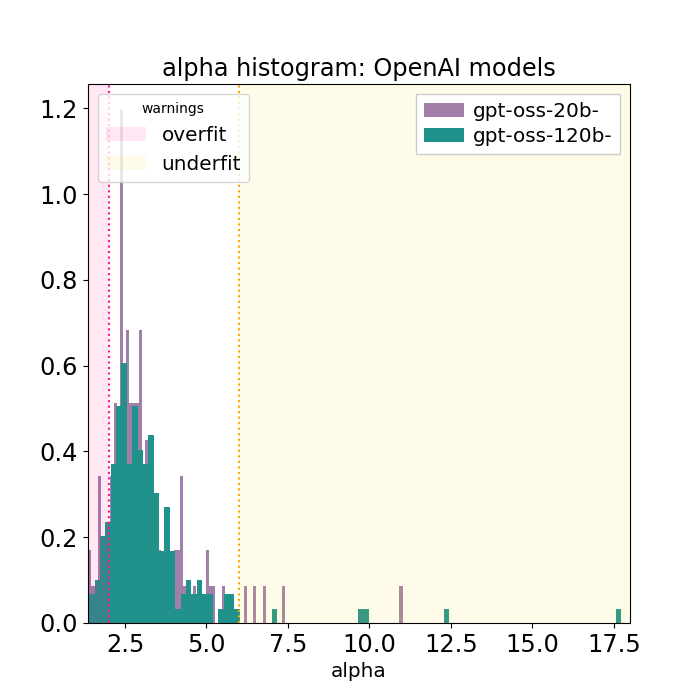
\includegraphics[width=0.48\columnwidth]{figures/oss_alpha_histogram.png}\hfill
\includegraphics[width=0.48\columnwidth]{figures/qwen25_alpha_histogram.png}
\caption{Layerwise HTSR $\alpha$ histograms from linear layers, computed with the open-source \WW~tool. Left: GPT-OSS 20B/120B models. Right: Qwen2.5 instruct models. The warning bands are heuristic: small $\alpha$ marks overfit or trap risk, while large $\alpha$ marks weakly correlated or underfit tails. Details and notebooks are listed in the appendix.}
\label{fig:alpha_histograms}
\vspace{-0.6em}
\end{figure}

\section{SETOL: the trace-log condition}
\label{sxn:setol}

\begin{tcolorbox}[marginalbox,title=\textbf{2. Phase-map summary}]
The best NN layers align the HTSR $\alpha=2$ with the SETOL trace-log law and ECS.
\begin{itemize}
\item HTSR identifies the power-law tail with $\alpha=2$.
\item SETOL identifies the ERG trace-log condition
\item Strong checkpoints make the two windows align.
\item Overfitting appears as traps or $\alpha<2$.
\end{itemize}
\takeaway{This alignment is a proposed RG signature.}
\end{tcolorbox}

SETOL is a \emph{Semi-Empirical Theory of Learning}.
It connects the layer empirical spectral density (ESD) to multilayer neural-network generalization accuracy using statistical mechanics,
providing a rigorous foundation for HTSR.
It is semi-empirical because it takes the layer ESD as empirical input and derives a layer-quality functional
whose diagnostics can be compared with the HTSR power-law metric $\alpha$.
In doing so, it assumes that a NN, near the optimal state of learning, satisfies a volume-preserving, scale-invariant transformation
(the trace-log condition) that resembles taking a single step of the Wilsonian Exact Renormalization Group (ERG)~\cite{WilsonKogut1974,Polchinski1984}.


SETOL starts by approximating the average generalization accuracy (one minus the error),
which it calls the average model quality $\overline Q_{\rm NN}$.
\begin{equation}
\overline Q_{\rm NN}\simeq 1-\overline E_{\rm gen}^{\rm NN}.
\label{eq:setol_quality}
\end{equation}
For a multilayer model, SETOL then approximates total model average quality by a product of layer contributions,
\begin{equation}
\overline Q_{\rm NN}\simeq\prod_{\rm layers}\overline Q_\ell .
\label{eq:setol_layer_product}
\end{equation}
Thus a layer quality $\overline Q_\ell$ estimates how much one layer supports the model's generalization accuracy.

Layer quality has a simple meaning here. It is one layer's contribution to generalization accuracy. A useful layer lowers error. A bad layer adds unstable gain or loses useful capacity.
This is the practical meaning of ``layer quality'' throughout the paper.

SETOL derives the layer quality using the layer-quality-squared generating function,
\begin{equation}
\begin{aligned}
\overline Q^{\,2}
&=\frac{1}{\beta}\frac{\partial}{\partial n}
  \left[\lim_{N\gg1}\beta\Gamma_{\overline Q^2}^{\rm IZ}\right] \\
&\simeq_{\rm high\text{-}T}
  \frac{1}{n}\frac{\partial}{\partial\beta}
  \left[\lim_{N\gg1}\beta\Gamma_{\overline Q^2}^{\rm IZ}\right] .
\end{aligned}
\label{eq:setol_q_derivative}
\end{equation}
Here $n$ is the sample count, and $\beta$ is the inverse-temperature parameter.
This is evaluated in the thermodynamic large-$n$ (and large-$N$) limit.
This generating function is essentially an effective layer free energy (up to sign convention).

SETOL then models each layer using a matrix generalization of the classic student-teacher perceptron~\cite{SeungSompolinskyTishby1992},
but now where the trained layer supplies the teacher matrix $\mathbf{T}=\mathbf{W}$ and is the fixed input.
The matrix free energy or generating function $\beta\Gamma_{\overline Q^2}^{\rm IZ}$
is formed by taking a thermal average over all possible students $\mathbf{S}$ that can
reproduce the outputs of the teacher layer (in an annealed approximation, and at high-T).
This gives an HCIZ integral
\begin{equation}
\begin{aligned}
\beta\Gamma_{\overline Q^2}
&=\frac{1}{N}\log\int d\mu(\widetilde{\mathbf A})
   \exp\{N\mathcal S(\widetilde{\mathbf A})\},\\
\mathcal S(\widetilde{\mathbf A})
&=n\beta\,\Tr\!\left[
   \frac{1}{N}\mathbf T^T\widetilde{\mathbf A}_{N}\mathbf T
   \right]
   +\frac{1}{2}\Tr\log(\widetilde{\mathbf A}_{M}) .
\end{aligned}
\label{eq:setol_hciz}
\end{equation}
When evaluated in the thermodynamic limit, and under an RG-like assumption,
this will depend only on the ESD of the layer (teacher) weight matrix.

\begin{tcolorbox}[marginalbox,title=\textbf{3. SETOL free energy and ERG trace-log}]
  Matrix-generalized statistical mechanics student-teacher model of NN generalization accuracy:
  \eqtight{
       1-\overline E_{\rm gen}^{\rm NN}\simeq
     \overline Q_{\rm NN}\simeq\prod_\ell \overline Q_\ell}
\begin{itemize}
\item \textbf{Layer Quality $\overline Q_\ell$:} one layer's contribution to total accuracy (1-error). Depends simply on $\X$.
\item \textbf{Effective Free Energy} $\beta\Gamma^{\rm eff}_{\overline Q^2}$ estimates $\overline Q_\ell$ with a random-matrix HCIZ integral
  \item \textbf{ERG scale fixing:} remove volume drift with
\eqtight{
  \Tr\log\Xtilde_{R}=0
  \qquad\Longleftrightarrow\qquad
  \det\Xtilde_{R}=1 .
}
\end{itemize}
\takeaway{SETOL says: relate the HTSR power-law fits to the generalization accuracy using the proposed Wilsonian Exact RG condition.}
\end{tcolorbox}

Here $\mathbf{T}$ is the empirical teacher layer.
The operator $\widetilde{\mathbf A}$ is the student correlation operator restricted to the Effective Correlation Space (ECS).
The subscripts $N$ and $M$ denote the compatible $N\times N$ and $M\times M$ forms of $\widetilde{\mathbf A}$.
The first term measures teacher-student alignment. It rewards a student spectrum that matches the trained layer.
The second term is the log-volume term.
It appears when the theory rewrites weight variables as correlation variables.
To evaluate the theory, we need to take a single step of the Wilsonian Exact Renormalization Group (ERG).


\begin{figure*}[t]
\centering
\safeincludegraphics[width=0.98\textwidth]{figures/fig3_spectral_flow.png}
\caption{
HTSR/SETOL phases during training. 
The HTSR power-law tail $\mathcal T_{\rm PL}$ and the SETOL Effective Correlation Space $\mathcal R_{\rm ECS}$ are selected independently.
During training, they overlap. At convergence, they align
$\mathcal R_{\rm ECS}^{\star}\simeq \mathcal T_{\rm PL}^{\star}$, at $\alpha\simeq2$.
}
\label{fig:spectral_flow_schematic}
\end{figure*}

The Wilsonian ERG step in SETOL is a change of variables and a change of scale. The bare layer variables are the student weights. The effective variables are the retained correlation modes in $\widetilde{\mathbf A}$. Section~\ref{sxn:setol} of the SETOL paper describes this step as an Effective-Hamiltonian construction: a bare layer Hamiltonian for $\overline Q^2$ is rewritten as a renormalized effective Hamiltonian on the ECS \cite{MartinHinrichsSETOL2025}.
\[
 d\mu(\mathbf S)\,e^{n\beta N\Tr\mathcal H_{\overline Q^2}}
 \ \xrightarrow{\rm ERG}\
 d\mu(\widetilde{\mathbf A})\,
 e^{n\beta N\Tr\mathcal H_{\overline Q^2}^{\rm ECS}} .
\]
The arrow here is a scale-invariant, volume-preserving transformation, and is
effectively taking a single step of the Wilsonian Exact RG (ERG).
It is from this convenient construction that the ERG trace-log condition emerges.

For this work, which considers the learning dynamics under a more complete RG lens,
the ERG trace-log condition removes volume drift while retaining scale.
The optimal ECS flow should approach a stable scale-balanced state near $\alpha\simeq2$.
After rescaling, SETOL defines
a volume-preserving scale-invariant transformation 
on the student $\widetilde{\mathbf A}$ and teacher $\Xtilde$ correlation matrices
\begin{equation}
\Tr\log\widetilde{\mathbf A}=0 \leftrightarrow \Tr\log\Xtilde_{\Rell}\simeq0 .
\label{eq:setol_trlog_AX}
\end{equation}
As shown here, the SETOL ERG trace-log law can be defined by dividing the retained operator by its geometric mean;
the tilde marks this normalization.
Also, we have added the  $\mathcal R$ to denote the retained ECS.

The layer quality (squared) is now expressed
simply in terms of the tail of the ESD of $\X$,
using the integrated R-Transform $R_{\X}(z)$~\cite{Zee1996}:
\begin{equation}
\overline{Q}^{2}
=
\sum_{\lambda_i\in\Rell}
\int_{\lambda^{+}}^{\lambda_i}
R_{\X}(x)\, dx
\label{eq:setol_Q}
\end{equation}
where $R_{\X}(z)$ is an analytic function chosen to model the PL tail
(and is analogous to a renormalized self-energy).

The link between HTSR and SETOL is summarized in 
Figure~\ref{fig:spectral_flow_schematic}.
The HTSR PL tail, denoted $\TPL$, starts at the red vertical line.
The SETOL ECS, $\RECS$, starts at the purple line.
The two tails are chosen independently and overlap during training.
At convergence, $\alpha=2$ and $\Tr\log\Xtilde_{\Rell}=0$,
they align: $\lambda^{+}_{\Rell}-\lambda^{+}_{\rm PL}\simeq 0$.
Also, (not shown) the truncated-SVD approximation  becomes exact for the test / generalization accuracy.

\begin{tcolorbox}[marginalbox,title=\textbf{4. ECS and PL tails during training}]
\begin{itemize}
\item \textbf{Underfit/ weak tail:} $\RECS\supset \TPL$.
\item \textbf{ERG Condition:} $\RECS^{\star}\simeq\TPL^{\star}$.
\item \textbf{Overfit / dominant tail:} $\RECS\subset\TPL$. 
\end{itemize}
\eqtight{\RECS^{\star}\simeq\TPL^{\star}.}
\takeaway{At the ERG condition, the ECS and PL tails align.}
\end{tcolorbox}


%Additionally, 
%truncated-SVD form and reproduce the test accuracy nearly perfectly.
%This is critical because it shows that the generalizing components of the layer have fully concentrated into the ECS.
%Finally, small experiments verify that when $\alpha<2$, the size of the ECS shrinks, correlation traps
%may form (defined below), and the test error degrades.\cite{PrakashMartinLateCollapse2026,PrakashMartinTraps2026}


%%%\begin{strip}\vspace{-0.35em}
%%%\centering
%%%\safeincludegraphics[width=0.98\textwidth]{figures/fig3_spectral_flow.png}
%%%\captionof{figure}{Schematic spectral flow for HTSR/SETOL training and overfitting. The Gaussian branch begins with a Marchenko--Pastur-like spectrum and no fitted power-law tail. Training then moves the layer through weakly and moderately heavy-tailed regimes. Red dashed lines mark the MLE/KS power law cutoff. Purple dashed lines mark the trace-log ECS cutoff. Strong checkpoints occur when the cutoffs nearly align near $\alpha\simeq2$. Overfitting can appear through correlation traps or by crossing into the very-heavy-tailed $\alpha<2$ regime.}
%%%\label{fig:spectral_flow_schematic}
%%%\vspace{-0.35em}\end{strip}
%%%
\clearpage

\section{The self-averaging boundary}
\label{sxn:selfavg}

Self-averaging is the concentration condition behind the trace law. When many eigencomponents contribute, a layer average becomes stable. When a few dominant tail components dominate, the average fails to concentrate. Figure~\ref{fig:self_average_schematic} shows this distinction in its simplest form.

\begin{tcolorbox}[marginalbox,title=\textbf{5. Self-averaging boundary}]
Self-averaging asks whether variance concentrates.
\begin{itemize}

\item \(\mathrm{Var}[X_M]\to 0\), a bound can be formed
\item \(\mathrm{Var}[X_M]=O(1)\), a bound is flat or vacuous.
\end{itemize}
\takeaway{The boundary is between vanishing variance and persistent \(O(1)\) variance.}
\end{tcolorbox}

\begin{figure*}[!b]
\centering
\safeincludegraphics[width=0.78\textwidth]{figures/self_averaging_schematic.png}
\caption{Self-averaging versus non-self-averaging. In the self-averaging case, individual samples concentrate around the mean, and the variance of the average shrinks with system size, allowing for concentration bounds. In non-self-averaging, the effective number of contributing eigencomponents stays small. The variance remains $O(1)$, so the bound becomes flat or vacuous.}
\label{fig:self_average_schematic}
\end{figure*}

Figure~\ref{fig:self_average_schematic} compares the difference between when the variance concentrates and a useful bound can be formed,
and where the variance remains finite in the infinite limit, preventing any useful bound from being defined.
In the self-averaging case, the effective number of contributing degrees of freedom grows with the layer width.
One can then form a Hoeffding-like concentration bound which shrinks with system size:
\begin{equation}
\Pr\{|X_N-\mathbb E X_N|>\epsilon\}
\lesssim \exp[-c\,M_{\rm eff}\epsilon^2],
\qquad M_{\rm eff}\to\infty .
\end{equation}
When the variance shrinks, the average becomes predictable. Moreover, one can sample from such a distribution
and expect to make reasonably reliable predictions on out-of-sample data.

In the non-self-averaging case, however, the effective number of contributors does not grow.
A few dominant tail components carry an $O(1)$ fraction of the trace. Then $M_{\rm eff}=O(1)$, and the same bound becomes
\begin{equation}
\Pr\{|X_N-\mathbb E X_N|>\epsilon\}
\lesssim \exp[-c\,O(1)\epsilon^2].
\end{equation}
One can form a bound and it may still be formally true, but it no longer improves with width.
It is flat. In practice, it can become vacuous. Concentration fails.
In such cases, one can describe in-sample data, but it is pointless to expect reliable predictions
on out-of-sample data, let alone out-of-distribution data.  

In an NN, for any given layer, the retained PL/ECS tail supplies the relevant components which can become
non-self-averaging and therefore modulate the generalization accuracy.
The dominant tail components mean the largest eigencomponents inside the retained power-law/effective-correlation tail, $\mathcal R\simeq\mathcal T_{\rm PL}$.
These are eigenvalue--eigenvector directions in the retained spectral tail.
The SETOL ERG trace-log condition gives the observable we want, the first spectral moment.
We elevate the trace-log to a trace-law. 
A self-averaging test then asks whether the remaining trace-law gain is spread across many eigencomponents or
concentrated in a few dominant tail components.

Section~\ref{sxn:tracelog} makes this precise, and explains how the $\alpha=2$ boundary arises
just from considering self-vs-non-self-averaging.
Section~\ref{sxn:saevidence} gives the empirical evidence that shows non-self-averaging
can predict overfitting even in the finite-size case of a NN layer.

\clearpage
\subsection{Trace-log and trace law}
\label{sxn:tracelog}
\begin{tcolorbox}[marginalbox,title=\textbf{6. Why $\alpha\simeq2$ is optimal}]
  The retained tail controls the first spectral moment:
    \eqtight{
      \widetilde E=M_R^{-1}\sum_{i\in\mathcal R}\lambda_i=\int \lambda\,\widehat\rho_R(\lambda)\,d\lambda
      }
\begin{itemize}
\item \textbf{$\alpha>2$:} stable, but the tail adds too little.
\item \textbf{$\alpha<2$:} a few top tail components dominate
\item \textbf{$\alpha\simeq2$:} the boundary between self- and non-self-averaging
\end{itemize}
\takeaway{$\alpha=2$ is the boundary between optimal learning and overfitting.}
  \end{tcolorbox}


The SETOL ERG trace-log condition~\eqref{eq:setol_trlog_AX} is the entry point for self-averaging
\begin{equation}                                                                                                                                         
\Tr\log\Xtilde_{\Rell}=0                                                                                                                                 
\qquad\Longleftrightarrow\qquad                                                                                                                          
\prod_{i\in\mathcal R}\widetilde\lambda_i=1.                                                                                                             
\end{equation} 
Here, we ask, when does the trace-log contain the maximum number of (generalizing) eigencomponents before
a few dominant tail components control it?

Self-averaging answers that question.
For a neural-network layer, we promote the trace-log to a \emph{Trace-Law}: the average spectral quality gain carried by the active eigencomponents.
\footnote{Here non-self-averaging refers to fluctuations of the trace-law observable, not the literal variance of the eigenvalue distribution.}
%Section~3 restricts the layer to an effective correlation space $\Rell$
%and removes its product scale:
%\begin{equation}
%\Tr\log\Xtilde_{\Rell}=0
%\qquad\Longleftrightarrow\qquad
%\prod_{i\in\mathcal R}\widetilde\lambda_i=1.
%\end{equation}
%This step does not make the layer good by itself; it fixes the scale and checks the ERG condition.
%that comes from multiplying all retained eigenvalues by the same constant. After this scale is removed, the remaining question concerns spectral shape.


%%%\begin{tcolorbox}[marginalbox,title=\textbf{5. Trace law: directional meaning}]
%%%Stable gain is well distributed gain.
%%%\eqtight{\mathbb E_u\!\left[u^T\X_{\Rell} u\right]=\frac{1}{\Mred}\Tr\X_{\Rell}.}
%%%\begin{itemize}
%%%\item \textbf{Meaning:} $M_{\Rell}^{-1}\Tr\X_{\Rell}$ is the average squared gain of the layer on a typical active direction.
%%%\item \textbf{Interpretation:} use it as a spectral proxy for the layer's quality contribution.
%%%\item \textbf{Test:} does this gain come from many eigencomponents, or a few dominant tail components?
%%%\end{itemize}
%%%\takeaway{If many eigencomponents share the gain, layer quality is stable. If a few dominate it, generalization performance can degrade.}
%%%\end{tcolorbox}
%%%


%Let $\Splus=\{i:\lambda_i>0\}$ denote the full positive spectral support,
%and let $\Rell\subseteq\Splus$ with $\Mred=|\Rell|$ denote a candidate retained effective space.
%The SETOL RG section below formalizes how this retained space is selected and rescaled; the present section only needs these symbols to state the self-averaging test.
The \emph{Trace-Law Gain or Energy} is
\begin{equation}
  E_+
  =\frac{1}{M}\Tr \X
=\frac{1}{M}\sum_{i\in\Splus}\lambda_i.
\label{eq:layerenergy}
\end{equation}

On the retained ECS $\Rell$, the corresponding energy is
\begin{equation}
  \Ered
  =\frac{1}{\Mred}\Tr \X_{\Rell}
  =\frac{1}{\Mred}\sum_{i\in\Rell}\lambda_i
=\int\lambda\,\rhohat_{\Rell}(\lambda)\dd\lambda.
\label{eq:Ered_prob}
\end{equation}
where $\Mred=|\Rell|$ denotes the candidate retained ECS dimension.

This is the first spectral moment.
It measures trace-law energy or gain: how much total gain the layer carries per active eigencomponent.
Equivalently, it measures the gain seen by a typical direction in the active space.
This also corresponds to a gain in layer quality and therefore model quality.

The self-averaging boundary says that spectral gain helps only when it is spread across enough eigencomponents for the layer average to concentrate. During training, a layer can increase its spectral norm as it learns, and it can also spread its eigenvalues into a broader retained tail. The trace law asks whether this extra gain is distributed across many effective eigencomponents or concentrated in a few dominant tail directions. When many components contribute, the variance of the layer average shrinks, the concentration bound improves with effective tail size, and the gain can support layer quality. When a few dominant tail components carry an O(1) share of the trace, the layer does not self-average. Fluctuations persist, the bound becomes flat or vacuous, and model error can stop improving or start growing. In this regime, larger spectral scale is not useful learned structure; it is tail-dominated instability, and generalization performance can degrade.


\medskip\noindent\textbf{Three regimes naturally emerge.}
According to HTSR, we know that retained eigenvalues can eventually be fit to a power law
\begin{equation}
\rho(\lambda)\sim C\lambda^{-\alpha}.
\label{eq:tailideal}
\end{equation}
Then the survival tail obeys
\begin{equation}
\Pr(\lambda>u)\sim C'u^{-\mu},
\qquad
\mu=\alpha-1.
\label{eq:mu}
\end{equation}
The index $\mu$ controls whether sums are supported by many terms or by the largest terms.


\medskip\noindent\textbf{Underfit regime:} If $\alpha>2$, equivalently $\mu>1$, then the first spectral moment is finite in the ideal model and
\begin{equation}
\sum_{i=1}^{M}\lambda_i\sim M\mathbb E[\lambda],
\qquad
\frac{\lambda_{\max}}{\sum_i\lambda_i}\to0 .
\label{eq:sa_alpha_gt_two}
\end{equation}
Many eigencomponents support the trace-law gain.


\medskip\noindent\textbf{Overfit regime:} If  $\alpha<2$, equivalently $\mu<1$, then
\begin{equation}
\sum_{i=1}^{M}\lambda_i=O(M^{1/\mu}),
\label{eq:sa_alpha_lt_two}
\end{equation}
and a few dominant tail components can carry an $O(1)$ fraction of the trace-law gain.
A few tail components can then dominate the layer.

\medskip\noindent\textbf{Boundary regime:} If  $\alpha=2$, or, equivalently $\mu=1$, the layer is at the  boundary between
optimal learning and overfitting.
This boundary gives the word ``optimal'' a precise operational meaning. A useful layer should capture as much structured variation (correlations/information) as possible.
Moving from large to smaller $\alpha$ strengthens the heavy tail and lets the layer represent more correlated structure.
But crossing below $\alpha=2$ makes the first spectral moment increasingly vulnerable to a few dominant tail eigenvalues.
The best checkpoint should therefore lie near the boundary, not deep on either side. This is a core prediction of the theory.

This is the HTSR phase boundary that matters for the paper (although the $\alpha=2$ is not specifically called out)
Still, in Bouchaud's heavy-tailed matrix theory, the corresponding $\mu=1$ case marks a special boundary between ordinary averaging and extreme-dominated sums \cite{CizeauBouchaud1994}. The SETOL RG section below argues that this HTSR boundary and the RG scale-balance boundary are the same boundary.

Simply put, for each layer, there is a natural boundary between effectively the tightest possible bound on the contribution to the
error and a phase where it is impossible to form a standard self-averaging bound.
That is when the HTSR $\alpha=2$. And at this boundary, the SETOL ERG trace-log law is the natural condition for
fixing scale.


\clearpage
\subsection{Empirical non-self-averaging}
\label{sxn:saevidence}
The self-averaging argument now needs an empirical test for real-world, finite-size neural networks.
A finite layer has crossed the self-averaging boundary when a small part of the retained tail starts to control the layer observable,
and, as predicted, is associated with a noticeable drop in the test accuracy of the model.
We use two warnings.  The first warning occurs when the HTSR power-law exponent drops into the overfitting regime, $\alpha<2$.
The second warning is what we call correlation traps (described below).
Both warnings have been observed previously and correlated with
drops in the test accuracy; we reproduce some of those results here~\cite{MartinHinrichsSETOL2025,PrakashMartinTraps2026,PrakashMartinLateCollapse2026}.

\begin{tcolorbox}[marginalbox,title=\textbf{7. Empirical evidence of non-self-averaging}]
Overfitting can leave two signatures in the weights:
\begin{itemize}
\item \textbf{$\alpha<2$:} the retained tail enters an extreme-dominated regime.
\item \textbf{Correlation Traps:} the randomized spectrum violates the MP/TW edge.
\item \textbf{Foundation scans:} low-$\alpha$ layers mark where trap tests are needed.
\end{itemize}
\takeaway{The warning is spectral: the loss can look acceptable while the layer stops self-averaging.}
\end{tcolorbox}

We start by looking at \emph{Correlation Traps}.
Given $\mathbf{W}$,  permute its entries $W_{ij}$ elementwise to form $W^\pi$.  This removes learned entrywise 
correlations while making the distribution $p(W_{i,j})$ i.i.d.
Then form the ESD of  $W^\pi$ and fit it to the MP baseline~\cite{MarchenkoPastur1967}.  Since the MP fit is deterministic, it is also the self-averaging baseline,
and significant deviations from this are also empirical evidence of non-self-averaging~\cite{PrakashMartinTraps2026,PrakashMartinLateCollapse2026}.

\begin{figure}[!h]
\centering
\safeincludegraphics[width=.75\columnwidth]{figures/traps.png}
\caption{Correlation traps.}
\label{fig:traps}
\vspace{-0.65em}
\end{figure}

A correlation trap is a large eigenvalue spike in the positive spectrum of $X^\pi$ beyond the MP/Tracy--Widom (TW) edge~\cite{MarchenkoPastur1967,TracyWidom1996}.
See Figure~\ref{fig:traps_alpha_evidence}.  The trap count is
\begin{equation}
N_{\rm trap}
=
\#\left\{i:\lambda_i(X^\pi)>\lambda_+^{\rm MP}+\Delta_{\rm TW}\right\},
\label{eq:trap_count}
\end{equation}
where $\Delta_{\rm TW}$ is the finite-size edge tolerance.  If $N_{\rm trap}>0$ persists across checkpoints, the layer has a correlation trap.
Figure~\ref{fig:traps} depicts a typical MP fit with several traps.

\begin{figure}[h]
\centering
\safeincludegraphics[width=\columnwidth]{figures/mlp_traps.png}
\caption{Empirical evidence for non-self-averaging in long-horizon grokking. After elementwise randomization of trained layer weights, one sees
persistent outliers beyond the MP edge, which appear as correlation traps. Trap counts rise as test accuracy degrades.
Reproduced from \cite{PrakashMartinLateCollapse2026}.}
\label{fig:traps_count_evidence}
\end{figure}


Figure~\ref{fig:traps_count_evidence} shows the mechanism in a long-horizon grokking run.  Test accuracy first rises and then collapses.  At the same time, randomized-spectrum outliers appear beyond the MP/TW edge.  The trap count then rises as held-out accuracy degrades.  This is the cleanest empirical picture of non-self-averaging: the model keeps training, but the retained spectral mass stops behaving like a stable average.

Traps and $\alpha<2$ are related, but they are not the same diagnostic.  A broad very-heavy tail can produce $\alpha<2$ without a single isolated trap.  Conversely, a trap can appear before the fitted exponent crosses two.  The two diagnostics therefore measure different ways for the layer to leave the self-averaging regime.

Figure~\ref{fig:traps_alpha_evidence} shows the layer average $\alpha$ dropping below two after trap structure has already appeared.
This order is important.  A trap can distort the ESD and harm the PL fit.
Thus $\alpha<2$ is a broad warning, while traps are a sharper MP-baseline violation.

\begin{figure}[!h]
\centering
\safeincludegraphics[width=\columnwidth]{figures/mlp_alphas.png}
\caption{Average HTSR exponent $\alpha$ for FC1 and FC2 during long-horizon grokking. The exponent falls below the critical value $\alpha=2$ as training progresses. Reproduced from \cite{PrakashMartinTraps2026}.}
\label{fig:traps_alpha_evidence}
\vspace{-0.65em}
\end{figure}

Together, these experiments give a finite-size test of self-averaging.  In healthy training, the retained spectral tail behaves like a stable layer average.  When this fails, it leaves signatures of overfitting in the layer weight matrices.

\clearpage
\begin{strip}\vspace{-0.55em}
\centering
\safeincludegraphics[width=0.95\textwidth]{figures/rg_flow_in_machine_learning_training.png}
\captionof{figure}{Operational RG flow for one dense layer. The step first decimates tiny-eigenvalue noise and retains an ECS tail $\mathcal R$. The SETOL-normalized retained eigenvalues are $\lambda_i/M$, and the retained dimension is $M_R=|\mathcal R|$. The trace-log condition fixes the product scale, $M_R^{-1}\sum_{i\in\mathcal R}\log(\lambda_i/M)=0$. The remaining trace-law gain is then tested for stable layer-quality contribution.}
\label{fig:rg_flow_energy}
\vspace{-0.75em}\end{strip}


\section{Wilsonian RG Flow}
\label{sxn:rg}
\vspace{0.35em}


\begin{tcolorbox}[marginalbox,title=\textbf{8. RG Flow}]
  RG describes the flow of the spectral density
  \eqtight{\mathcal{R}_{\mathrm{RG}}:\rho(\lambda)\longrightarrow \rho_{\rm tail}^{*}(\lambda).}
  \takeaway{The RG flow encodes how the spectral density $\rho(\lambda)$ approaches a candidate fixed point,
    satisfying both the HTSR $\alpha\simeq 2$ and the SETOL trace-log law.}
\end{tcolorbox}

This section describes a Wilsonian RG construction for the
spectral density $\rho(\lambda)$ as the heavy-tailed power-law density forms
and approaches the HTSR $\alpha=2$ candidate optimal state under the SETOL trace-log law.
It is the shape, not the scale, that regulates the final layer quality and therefore the final model generalization accuracy.
The retained layer should help accuracy improve, or equivalently help error decrease,
without making the layer contribution explode or collapse. 
Trace-log normalization removes arbitrary scale.
The RG construction shows when the spectral shape collapses, diverges, or converges.

The goal here  is to identify an effective description of a trained
layer--the Effective Correlation Space (ECS)--by repeatedly removing
small-scale spectral components, retaining the dominant
correlation structure, and eliminating redundant overall scale.
Rather than develop a formal RG map, we describe the
construction operationally using a truncated-SVD picture
together with explicit trace-log renormalization. The resulting
flow acts on the retained spectral density (in the ECS)
and motivates the HTSR $\alpha=2$ as the boundary between
learning and overfitting.

Figure~\ref{fig:rg_flow_energy} depicts the RG operational training flow. 
The practical picture is a truncated-SVD picture. An RG step keeps the spectral directions that matter for the learned correlation structure, drops directions that do not matter at the current scale, and rescales the retained layer.  Both growth of the spectral norm (scale) and growth of the spectral spread (shape) are therefore the same kind of effect: both change how strongly the layer amplifies retained directions.

In either view, both HTSR and SETOL play a critical role in both motivating the RG analysis here and providing the starting concepts and tools.

\subsection{HTSR phases and RG}
\label{sxn:htsr_rg}

HTSR provides the empirical starting point for the RG analysis.
Section~\ref{sxn:htsr} described trained layer spectra using HTSR heavy-tailed universality classes.
Here we use those classes as a coarse description of training flow.
We do not start with a microscopic model of the data, the optimizer, or the architecture.
We start with the observed fact that trained layer ESDs often become heavy-tailed power-law.

\begin{center}
\small
\setlength{\tabcolsep}{2.5pt}
\renewcommand{\arraystretch}{1.06}
\captionof{table}{HTSR classes interpreted as an RG flow.}
\label{tab:htsr_rg_flow}
\begin{tabularx}{\linewidth}{@{}lcc@{}}
\toprule
Phase & Exponent & RG meaning \\
\midrule
Random-like / Bulk+Spikes & no PL fit & Gaussian branch \\
Weakly HT & $\alpha\gg2$ & weak-energy sector \\
Moderately HT & $\alpha>2$ & approach to boundary \\
Strongly HT & $\alpha\simeq2$ & balanced boundary \\
Very HT / traps & $\alpha<2$ & dominant-tail sector \\
\bottomrule
\end{tabularx}
\end{center}

Table~\ref{tab:htsr_rg_flow} labels the HTSR phases, and Figure~\ref{fig:rg_flow_energy} shows how a layer moves through them. Training starts with many tiny-eigenvalue modes and a weak or steep tail, then retains an ECS tail and moves the ESD toward a more structured heavy-tailed spectrum.
The trace-law energy $\Ered$ from Section~\ref{sxn:tracelog} gives this motion its learning meaning:
for $\alpha>2$ the retained energy is weak and can collapse (orange panel),
near $\alpha\simeq2$ it remains balanced across scales (green panel),
and for $\alpha<2$ a few dominant tail modes can carry too much energy and drive the overfit regime (red panel)
where the energy diverges.

%%%Figure~\ref{fig:rg_flow_energy} shows this flow operationally.
%%%The top row begins with many tiny-eigenvalue modes and a weak or steep tail.
%%%Training trims the small modes, retains an ECS tail, and moves the ESD toward a more structured heavy-tailed spectrum.
%%%In the favorable case, the fitted exponent decreases toward $\alpha\simeq2$ and the retained spectrum reaches the balanced panel on the right.
%%%If the flow continues past this boundary, the layer can enter the red overfit regime, where a few dominant tail modes control the energy.
%%%
%%%The trace-law energy $\Ered$ from Section~\ref{sxn:tracelog} gives these phases a simple meaning.
%%%For $\alpha>2$, the retained energy is spread over weak tail modes and can collapse, as in the orange panel of Figure~\ref{fig:rg_flow_energy}.
%%%Near $\alpha\simeq2$, the retained energy stays balanced across scales, as in the green panel.
%%%For $\alpha<2$, a few dominant modes can carry too much energy, as in the red panel.
%%%
\begin{figure}[h]
\centering
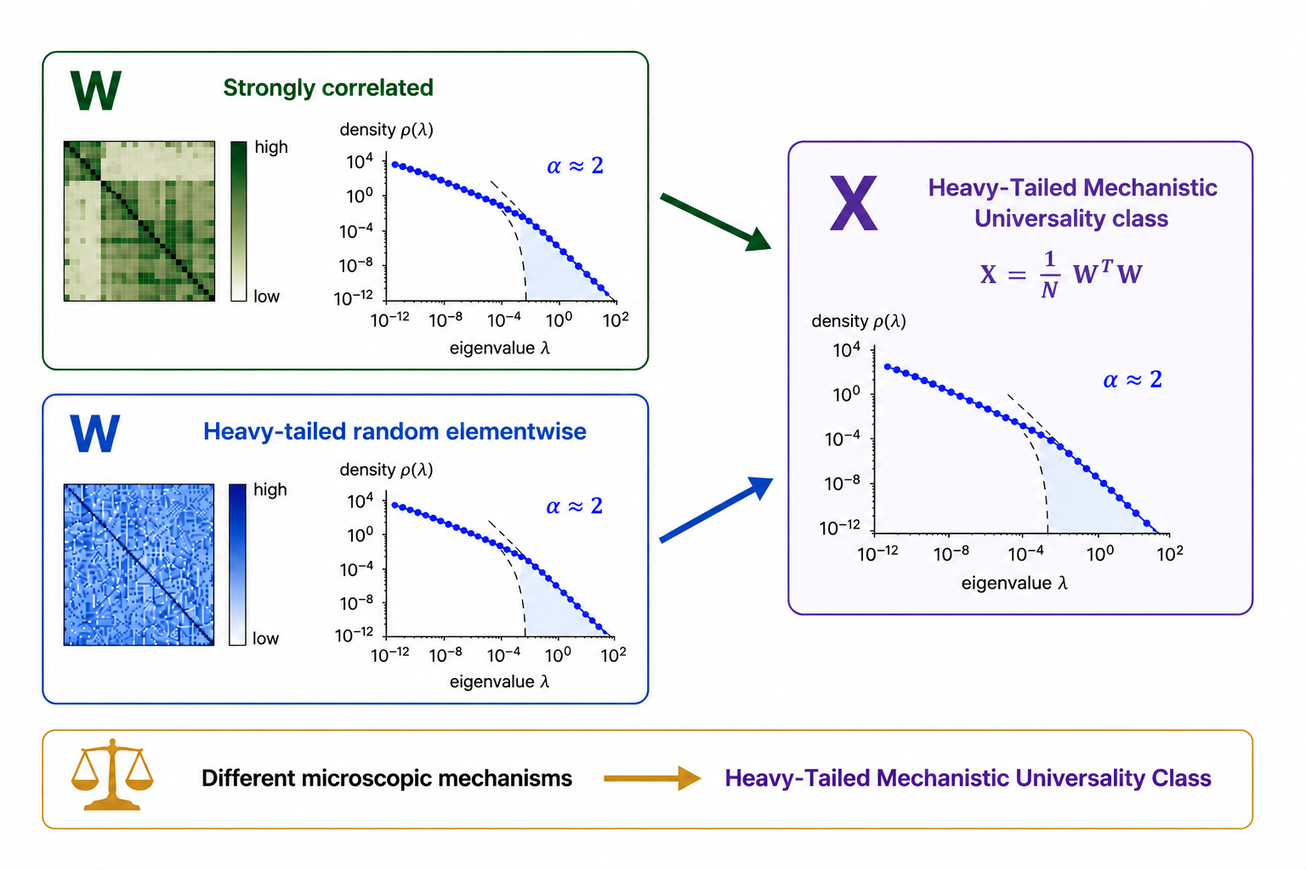
\includegraphics[width=\columnwidth]{figures/HT-MU.png}
\caption{\textbf{Heavy-Tailed Mechanistic Universality.}}
\label{fig:ht_mechanistic_universality}
\vspace{-0.6em}
\end{figure}

HTSR calls this \emph{Mechanistic Universality}.
Different architectures, datasets, and optimizers can produce the same heavy-tailed spectral endpoint.
This universality is spectral, not elementwise.
It is a property of the ESD of the correlation matrix $\X=N^{-1}\W^T\W$, not from a
Pareto distribution of entries $W_{ij}$. 
Indeed, the entries are generally not HT; learned correlations can make the spectrum heavy-tailed.
Here we interpret this mechanistic universality as a preview of RG universality:
different microscopic training dynamics can flow toward the same coarse-grained spectral behavior.
To connect this to renormalization group universality, SETOL supplies the bridge.

\newpage

\subsection{SETOL and RG}
\label{sxn:setol_rg}

SETOL contributes the scale convention for the RG analysis.
Section~\ref{sxn:setol} introduced the layer quality generating function, an effective free energy  $\beta\Gamma^{\rm eff}_{\overline Q^2}$
and showed that the Wilsonian ERG construction leads to the ERG trace-log condition.
The present paper does not need to evaluate the full SETOL quality $\overline{Q}$.
Instead, we use the ERG trace-log condition to define the scale,
and we study the flow of the retained trace-law energy $\Ered$ on that scale.

\begin{tcolorbox}[marginalbox,title=\textbf{9. SETOL $\rightarrow$ RG energy flow}]
\small
\textbf{Energy object:}
\[
\Ered=\frac{1}{\Mred}\Tr\XR
=\int \lambda \rhohat_{\Rell}(\lambda)\,d\lambda .
\]
\textbf{Scale fixing:}
\[
\Tr_{\Rell}\log\Xtilde_{\Rell}=0 .
\]
\textbf{Band energy gain:}
\[
G_E(\Lambda,b)
=
\int_{\Lambda}^{b\Lambda}\lambda\,\rhohat_{\Rell}(\lambda)\,d\lambda .
\]
\takeaway{RG studies how the retained trace-law energy flows across spectral scales.}
\end{tcolorbox}

Figure~\ref{fig:rg_flow_energy} shows RG decimation, rescaling, and the resulting energy flow. The trace-log is the scale-fixing operation;
it is not itself the flowing energy. The quantity whose flow we study is the retained trace-law energy $\Ered$,
rescaled as needed.
Section~\ref{sxn:tracelog} defined this energy as the first moment of the retained ECS.
The RG question is therefore concrete: after the trace-log removes arbitrary product scale,
how does $\Ered$ flow across spectral scales?

We answer this question by using the trace-log to measure covariance volume. On the retained positive spectrum,
\begin{equation}
\Tr\log\X_{\Rell}
=
\log\det\X_{\Rell}
=
\sum_{i\in\Rell}\log\lambda_i .
\end{equation}
Thus the trace-log measures the logarithm of the retained covariance volume. It does not add eigenvalue gains directly;
it measures their product scale.
Once fixed, the natural comparison is across fixed-ratio bands $[\Lambda,b\Lambda]$,
or equivalently across equal-width intervals in $\log\lambda$.

We therefore study how much retained layer energy lies in each spectral band. Define the band energy gain
\begin{equation}
G_E(\Lambda,b)
=
\int_{\Lambda}^{b\Lambda}
\lambda\,\widehat\rho_{\Rell}(\lambda)\,d\lambda .
\end{equation}
This is the portion of the retained trace-law energy carried by the logarithmic band $[\Lambda,b\Lambda]$. If $G_E(\Lambda,b)$ decreases as the band moves to larger eigenvalues, the retained tail is weak. If it increases, the layer is moving toward dominant-tail concentration. If it remains comparable across bands, the spectrum is scale-balanced.

The next subsection shows that the HTSR power-law tail $\rho_{\rm tail}(\lambda)$ makes the energy gain stable at $\alpha=2$.
That is, we illustrate that $\alpha$ is analogous to an RG universal critical exponent.

\clearpage

\subsection{Effective description during training}
\label{sxn:effdescr}
We can now organize these concepts around the Wilsonian RG framework, leveraging the HTSR empirical observations and the  SETOL trace-log condition.
For a practitioner, this is the same controlled truncated-SVD flow stated in the box. First choose a retained spectral space.
Then form the effective layer on that space. Then divide out the retained geometric-mean scale. Finally compare the remaining spectral shape.

\begin{tcolorbox}[marginalbox,title=\textbf{10. RG step as ECS/SVD projection}]
The generalizing components concentrate in a low-rank subspace
  \begin{itemize}
\item \textbf{Truncate:} keep the retained ECS eigenspace
\eqtight{
X_{\Rell}=\U_{\Rell}^\top X \U_{\Rell}
      =\operatorname{diag}\{\lambda_i:i\in\mathcal R\}.
}
\item \textbf{Rescale:} by the geometric-mean eigenvalue
\eqtight{
\widetilde X_{\Rell}=\frac{X_{\Rell}}{\lambda_g^{(\mathcal R)}},
\qquad
\lambda_g^{(\mathcal R)}
=
\exp\!\left(
\frac{1}{|\mathcal R|}
\sum_{i\in\mathcal R}\log\lambda_i
\right).
}
\item \textbf{Check:} after normalization,
\eqtight{
\Tr_{\mathcal R}\log\widetilde X_{\Rell}
=
\sum_{i\in\mathcal R}\log\widetilde\lambda_i
=
0.
}
\end{itemize}
  \takeaway{The final ECS contains all the information necessary to generalize to out-of-sample data.}
\end{tcolorbox}


This RG map separates the spectral flow into two effects, shape and scale.
As the retained layer shape changes, we identify which singular directions the layer uses and how broad the tail becomes.
We rescale the retained layer because changes in scale can make the accuracy contribution unstable.
The trace-log condition removes that scale before the final fixed-point test, $\alpha\simeq 2$. 

The SETOL ERG trace-log condition says that the learned effective space has a stable log-volume.
During training, the raw trace-log coordinate can settle to a plateau,
\begin{equation}
T_+(t)=\frac{1}{M_+}\Tr_{+}\log\X_+(t)
=\frac{1}{M_+}\sum_{i\in\Splus}\log\lambda_i(t),
\label{eq:setol_raw_plateau_T}
\end{equation}
with
\begin{equation}
T_+(t)\to T_+^\star,
\qquad
\Delta_t T_+\to0 .
\label{eq:setol_raw_plateau}
\end{equation}
The plateau need not be zero. Zero appears only after the retained space is normalized by the geometric mean eigenvalue $\lambda_g^{(\mathcal R)}$
(in SETOL, this is implicitly $\tfrac{1}{M}$).

The box separates three operations. The factor $1/N$ puts the layer in SETOL/RMT correlation units. The set $\mathcal R$ selects the retained ECS. This is the decimation step. It is like keeping the useful singular directions in a truncated-SVD and ignoring directions that carry negligible quality gain at the current scale. The scale $\lambda_g^{(\mathcal R)}$ then removes the product scale of the retained ECS.
%Dividing $\X_{\Rell}$ by $\lambda_g^{(\mathcal R)}$ is the same as dividing the effective weight matrix $\W_{\Rell}$ by $\sqrt{\lambda_g^{(\mathcal R)}}$.

Take note of one important normalization convention.  SETOL tests the trace-log condition on eigenvalues after the fixed layer-scale normalization by $M$.  Thus the empirical SETOL test uses $\lambda_i/M$, not raw $\lambda_i$ alone.  The retained count is $M_{\Rell}=|\mathcal R|$; this count sets the geometric mean over the retained ECS.  We use $M_{\Rell}$ throughout for the retained ECS dimension; it is a count, not a rescaled or normalized quantity.

The ECS construction therefore separates selection from rescaling. Selection chooses the retained spectral eigencomponents. Rescaling removes the arbitrary layer scale. The RG map then compares the remaining spectral shape. This is where the theory asks whether spectral-norm growth and spectral spread improve layer quality in a controlled way.  In RG language this is also called \emph{removing redundant directions and/or gauge fixing}.

The full positive spectrum gives the starting point. At the trivial Gaussian branch, no correlated tail has been selected. The natural support is therefore the full positive spectrum
\begin{equation}
\Splus=\{i:\lambda_i>0\},
\qquad
M_+=|\Splus|.
\label{eq:Splus}
\end{equation}
The full branch has trace-log coordinate
\begin{equation}
T_+(t)=\frac{1}{M_+}\Trplus\log \Xplus(t).
\label{eq:Tplus_intro}
\end{equation}
This coordinate describes the product-of-eigenvalues scale of the full positive spectrum (i.e., the determinant form of the trace-log law).

As training progresses, we expect that the layer generalizing eigencomponents will concentrate into a lower-rank subspace.
Therefore, the correlated branch uses a smaller effective space. Let $\Rell\subseteq\Splus$ be a candidate Effective Correlation Space and let
\begin{equation}
\Mred=|\Rell| .
\label{eq:mreddef}
\end{equation}
Note that $\Mred$ is not known before the construction. It changes as the spectral description is decimated to the eigencomponents that carry learned correlations.
Also, note that in this construction we ignore the null space of the layer, although it might also carry information in a multi-layer NN as it may cause one layer
to ``forget'' the correlations learned in a previous layer.

The RG-like flow acts on spaces and operators together. At step $n$, the retained object is the pair
\begin{equation}
\left(\mathcal R^{(n)},\,\X_{\Rell}^{(n)}\right),
\qquad
\Mred^{(n)}=|\mathcal R^{(n)}|.
\label{eq:flowpair}
\end{equation}
A decimation step removes eigencomponents that do not belong to the current correlated description.
A rescaling step then removes the product-of-eigenvalues scale on the retained eigencomponents.
The dimension $\Mred$  can and will therefore change from step to step until it eventually converges and captures
all of the generalizing components.

The ECS rule is operational. It searches over retained spectral spaces, normalizes each candidate by its geometric mean, and keeps a space whose normalized spectral shape remains stable under decimation. This paper uses that SETOL/ECS space as an input. It then tests whether the stable ECS matches the independently fitted HTSR power-law tail. The match is the key empirical claim, not a consequence of the normalization alone.

For a fixed retained space, the restricted operator is easy to write. Let $\U_{\Rell}$ be the matrix whose columns are the retained eigenvectors. Then
\begin{equation}
\X_{\Rell}=\U_{\Rell}^T\X\U_{\Rell}
=\diag(\lambda_i:i\in\Rell).
\label{eq:restricted_operator}
\end{equation}
The corresponding effective weight matrix is
\begin{equation}
\W_{\Rell}=\W\U_{\Rell},
\qquad
\X_{\Rell}=\frac{1}{N}\W_{\Rell}^T\W_{\Rell} .
\label{eq:effective_weight}
\end{equation}
This is the truncated-SVD view of the same operation. The retained columns of $\U_{\Rell}$ define the effective input directions. The matrix $\W_{\Rell}$ is the layer restricted to those directions.

The probability empirical spectral density on this retained space is
\begin{equation}
\rhohat_{\Rell}(\lambda)=\frac{1}{\Mred}\sum_{i\in\Rell}\delta(\lambda-\lambda_i),
\qquad
\int\rhohat_{\Rell}(\lambda)\dd\lambda=1.
\label{eq:prob_esd}
\end{equation}
With this convention, retained-space gain integrals are averages. If a counting density is used instead, every averaged trace-law integral must include a prefactor $1/\Mred$.

\begin{tcolorbox}[marginalbox,title=\textbf{11. The trace-log scale convention}]
Be careful; keep track of the normalization
\eqtight{M=\text{SETOL scaling},\;\;M_{\Rell}=|\mathcal R|=\text{Retained ECS}.} 
\eqtight{\lambda_i^{\rm SETOL}=\frac{\lambda_i}{M}.}
\eqtight{\frac{1}{M_{\Rell}}\sum_{i\in\mathcal R}\log\!\left(\lambda^{\rm SETOL}_i\right)\simeq0.}
\eqtight{\lambda_g^{(\mathcal R)}=\left(\prod_{i\in\mathcal R}\lambda_i\right)^{1/M_{\Rell}}\simeq M.}
\takeaway{SETOL eigenvalues have geometric mean $1$; the raw retained eigenvalues have geometric mean $M$.}
\end{tcolorbox}


The trace-log coordinate is the log of a geometric mean.  To match the SETOL convention, first use the fixed layer-scale normalization by $M$ and define
\begin{equation}
\X_{\Rell}^{\rm SETOL}:=\frac{\X_{\Rell}}{M},
\qquad
\widetilde\lambda_i^{\rm SETOL}:=\frac{\lambda_i}{M},
\qquad
M_{\Rell}:=|\mathcal R| .
\label{eq:setol_normalized_operator}
\end{equation}
On the retained space, the SETOL trace-log coordinate is
\begin{equation}
T_{\Rell}^{\rm SETOL}
=\frac{1}{M_{\Rell}}\Tr\log \X_{\Rell}^{\rm SETOL}
=\frac{1}{M_{\Rell}}\sum_{i\in\Rell}\log\widetilde\lambda_i^{\rm SETOL}.
\label{eq:Traw_precise}
\end{equation}
The empirical SETOL trace-log condition is
\begin{equation}
T_{\Rell}^{\rm SETOL}\simeq0
\qquad\Longleftrightarrow\qquad
\left(\prod_{i\in\Rell}\widetilde\lambda_i^{\rm SETOL}\right)^{1/M_{\Rell}}\simeq1 .
\label{eq:setol_trace_log_condition}
\end{equation}
Equivalently, the raw retained eigenvalues have geometric mean
\begin{equation}
\lambda_g^{(\mathcal R)}
:=\left(\prod_{i\in\Rell}\lambda_i\right)^{1/M_{\Rell}}
=\exp\!\left(\frac{1}{M_{\Rell}}\sum_{i\in\Rell}\log\lambda_i\right)
\simeq M .
\label{eq:geommean_precise}
\end{equation}
Thus the geometric mean is one for SETOL-normalized eigenvalues $\widetilde\lambda_i^{\rm SETOL}=\lambda_i/M$, and it is $M$ for the raw retained eigenvalues at the SETOL trace-log point.

For shape comparisons after this test, it is convenient to form the unit-geometric-mean retained operator
\begin{equation}
\Xtilde_{\Rell}=\frac{\X_{\Rell}}{\lambda_g^{(\mathcal R)}},
\qquad
\widetilde\lambda_i=\frac{\lambda_i}{\lambda_g^{(\mathcal R)}}.
\label{eq:Xtilde_precise}
\end{equation}
Equivalently, the normalized effective weight matrix is
\begin{equation}
\widetilde\W_{\Rell}=\frac{\W_{\Rell}}{\sqrt{\lambda_g^{(\mathcal R)}}},
\qquad
\Xtilde_{\Rell}=\frac{1}{N}\widetilde\W_{\Rell}^T\widetilde\W_{\Rell} .
\label{eq:Wtilde_precise}
\end{equation}
By construction,
\begin{equation}
\boxed{\Tr\log\Xtilde_{\Rell}=0.}
\label{eq:trlog_exact}
\end{equation}
This last equation is a shape-normalization identity.  The empirical SETOL test is the preceding statement that the SETOL-normalized retained eigenvalues $\widetilde\lambda_i^{\rm SETOL}=\lambda_i/M$ have geometric mean one.  The retained dimension $M_{\Rell}=|\mathcal R|$ is the denominator in the retained geometric mean; the fixed $M$ is the layer-scale normalization inherited from SETOL, which is implicit in the formulation.

The fixed-point object is therefore not the raw operator $\X_{\Rell}$ but rather is the normalized spectral shape of $\Xtilde_{\Rell}$, or equivalently of $\widetilde\W_{\Rell}$.
A fixed point means that this shape remains stable after further decimation and trace-log rescaling.
In practical terms, the retained layer keeps giving a controlled quality contribution after we remove arbitrary scale (i.e., during optimization with Muon).

The empirical claim is that two independently defined spaces align. The trace-log/ECS procedure identifies the retained
effective space $\mathcal R_{\rm ECS}^\star$.
A power-law fit identifies a finite-window tail $\mathcal T_{\rm PL}^\star$. At the proposed RG fixed point, the theory predicts
\begin{equation}
\boxed{\mathcal R_{\rm ECS}^\star\simeq\mathcal T_{\rm PL}^\star .}
\label{eq:alignment_claim}
\end{equation}
or, explicitly, in terms of the ECS/tail eigenvalues,
\begin{equation}
\rho_{\rm tail}(\lambda)\sim \lambda^{-2}\quad\text{and}\quad\sum_{\rm tail}\log\tilde{\lambda} \simeq 0.
\label{eq:alignment_practical}
\end{equation}

This alignment is not a definition. It is a measurable agreement between the trace-log effective space and the fitted heavy-tailed window.

Moreover, SETOL and thus our RG construction here also predict that at the proposed RG fixed point,
we can replace $\mathbf{W}\rightarrow \mathbf{W}_{R}$ (i.e., the truncated-SVD of $\mathbf{W}$),
with no degradation of the generalization / test accuracy.
This has been confirmed experimentally for small experiments (i.e. a 3-layer MLP on MNIST).

\clearpage
\subsection{RG Scale counting}
\label{sxn:rgcount}

RG scale counting asks how the layer-quality contribution changes as we move
across spectral scales. In an RG description, the spectrum is not treated as a
flat list of eigenvalues. It is grouped into scale bands $[\lambda, b\lambda]$ that are
natural for a power-law distribution.  Then we ask whether each
band contributes a stable amount after the RG rescaling step, or if the gain collapses/diverges.

\begin{tcolorbox}[marginalbox,title=\textbf{12. RG boundary}]
RG counts gain by scale.
\eqtight{G_E(\Lambda,b)=\int_\Lambda^{b\Lambda}\lambda\rho(\lambda)\,d\lambda.}
\eqtight{\rho(\lambda)=C\lambda^{-\alpha},\qquad \alpha=2\Rightarrow G_E(\Lambda,b)=C\log b.}
\begin{itemize}
\item \textbf{$\alpha>2$:} larger bands contribute less and less gain.
\item \textbf{$\alpha=2$:} each log band contributes the same gain.
\item \textbf{$\alpha<2$:} gain concentrates into a few large tail components, diverging.
\end{itemize}
\takeaway{$\alpha\simeq2$ is the log-scale-balanced boundary.}
\end{tcolorbox}

One RG step is a spectral operation in this paper. It discards eigencomponents outside the current effective description. It rescales the retained operator by its geometric mean. It then compares the normalized spectral shape with the previous retained shape. A fixed point means this decimate-and-normalize operation no longer changes the retained spectral shape or layer-quality gain.

The word ``exact'' is narrow here. It refers to a proposed Wilsonian map on the retained spectral distribution, not to a closed-form solution of the full network dynamics. We identify the candidate boundary and the candidate fixed-point signature of this map. It does not claim that one finite checkpoint exactly solves the full RG flow.

\begin{table*}[t]
\centering
\caption{Scale counting, statistics, and empirical meaning of the three spectral regimes.}
\label{tab:regimes}
%\scriptsize
\footnotesize
\setlength{\tabcolsep}{4pt}
\renewcommand{\arraystretch}{1.15}
\begin{tabularx}{\textwidth}{@{}p{0.085\textwidth}@{\hspace{0.5em}}p{0.19\textwidth}p{0.23\textwidth}p{0.245\textwidth}X@{}}
%\begin{tabularx}{\textwidth}{@{}p{0.10\textwidth}p{0.20\textwidth}p{0.24\textwidth}p{0.22\textwidth}X@{}}
\toprule
Regime & Trace-law gain per scale & Scale-flow meaning & Statistical meaning & Learning meaning \\
\midrule
$\alpha>2$ & $\lambda^2\rho(\lambda)\sim\lambda^{2-\alpha}\to0$ & Trace-law band gain decays; weak-tail sector or approach toward $\Fzero$. & First moment self-averages; dominant tail components stay controlled. & Stable but potentially weakly correlated or undertrained tail. \\
$\alpha=2$ & $\lambda^2\rho(\lambda)\sim\lambda^0$ & Scale-balanced logarithmic-band state; candidate $\Fhtsr$ when ECS aligns with the fitted tail. & Marginal self-averaging boundary. & Maximal stable structured-variation capture before tail-component domination. \\
$\alpha<2$ & $\lambda^2\rho(\lambda)\sim\lambda^{2-\alpha}\to\infty$ & Trace-law band gain grows toward the dominant tail components. & A few dominant tail components can dominate the first moment. & Overfit risk; correlation traps; held-out degradation. \\
\bottomrule
\end{tabularx}
\vspace{-0.25em}
\end{table*}

The fixed point is layerwise. We do not posit one global fixed point for an entire multi-layer network. Rather, each layer has its own spectrum, its own retained ECS, and its own proposed Wilsonian-style spectral fixed point. A strong checkpoint is therefore a coordinated network state in which the matrix-like layers sit near their own SETOL ERG fixed points.

Because the spectral density $\rho(\lambda)$ is heavy-tailed power law for a well-trained
layer, the natural RG scale band is logarithmic in $\lambda$, and the natural coordinate is
\begin{equation}
x=\log\lambda.
\end{equation}
A fixed-width interval in $x$ is a fixed-ratio spectral shell $\lambda\in[\Lambda,b\Lambda]$.
This is the spectral analogue of coarse-graining by length scale in ordinary
RG. Each logarithmic band asks how much trace-law gain is contributed by one
multiplicative decade of eigenvalues.


The object being counted is retained trace-law gain. With the probability ESD in Eq.~\eqref{eq:prob_esd},
\begin{equation}
\Ered=\int\lambda\,\rhohat_{\Rell}(\lambda)\dd\lambda.
\label{eq:E_continuum}
\end{equation}
Since $\dd\lambda=\lambda\dd\log\lambda$,
\begin{equation}
\dd\Ered=\lambda\rhohat_{\Rell}(\lambda)\dd\lambda
=\lambda^2\rhohat_{\Rell}(\lambda)\dd\log\lambda.
\label{eq:shell_dE}
\end{equation}
Thus the trace-law gain per logarithmic spectral scale is
\begin{equation}
\frac{\dd\Ered}{\dd\log\lambda}=\lambda^2\rhohat_{\Rell}(\lambda).
\label{eq:shellenergy}
\end{equation}
The factor $\lambda^2\rhohat_{\Rell}(\lambda)$ has a simple origin. One factor of $\lambda$ comes from the trace-law gain carried by an eigenvalue. The second factor of $\lambda$ comes from changing variables from linear spectral measure to logarithmic spectral measure, $\dd\lambda=\lambda\dd\log\lambda$. Thus $\lambda^2\rhohat_{\Rell}(\lambda)$ is just the trace-law gain per logarithmic spectral shell. Substituting $\rhohat_{\Rell}(\lambda)\simeq C\lambda^{-\alpha}$ then gives $C\lambda^{2-\alpha}$, so $\alpha=2$ is precisely the case in which each multiplicative spectral shell contributes the same trace-law gain.
In the RG sense, we say \emph{$\alpha=2$ is marginal}.

This quantity answers an interpretable question: how much of the retained layer's quality gain, and therefore how much of its possible accuracy contribution, lives near this multiplicative eigenvalue scale?

A power-law tail makes the answer transparent. If
\begin{equation}
\rhohat_{\Rell}(\lambda)\simeq C\lambda^{-\alpha}
\end{equation}
on the fitted finite window, then
\begin{equation}
\frac{\dd\Ered}{\dd\log\lambda}
\sim C\lambda^{2-\alpha}.
\label{eq:shellpower}
\end{equation}
When $\alpha>2$, high-eigenvalue shells carry less trace-law gain with scale. The retained layer may be stable but weak. When $\alpha<2$, high-eigenvalue shells carry more trace-law gain with scale. The largest retained directions can dominate the layer contribution. When $\alpha=2$, each logarithmic shell carries comparable trace-law gain. This is the scale-balance condition.

\begin{table*}[t!]
\centering
%\scriptsize
\footnotesize
\setlength{\tabcolsep}{5pt}
\renewcommand{\arraystretch}{1.05}
\caption{Special RG notation used in this section.}
\label{tab:rgterms}
\begin{tabularx}{\textwidth}{@{}p{0.16\textwidth}p{0.24\textwidth}X@{}}
\toprule
Term & Notation & Meaning here \\
\midrule
RG step &
$\mathcal R_{\rm ECS}$ &
Project to the retained ECS and rescale the ESD. \\

Fixed point &
$\mathcal R_{\rm RG}[\rho^\star]=\rho^\star$ &
A normalized ESD that is unchanged by the RG step. \\

Branch &
$\Fzero,\ \Fhtsr$ &
A family of normalized ESDs with the same qualitative RG behavior. \\

Weak-tail branch &
$\Fzero,\quad g_E^\star=0$ &
The trivial solution.  HTSR random-like phase and potentially nearby ESDs. \\

Correlated branch &
$\Fhtsr$ &
The empirical RG fixed point candidate. \\

Beta function &
$\beta_E(g_E)=d g_E/d\log\lambda$ &
The scale derivative of the trace-law gain. For a PL tail, $\beta_E(g_E)=(2-\alpha)g_E$. \\

Energy &
$\overline E=\Ered/\lambda_g$,\quad $g_E=d\overline E/d\log z$ &
Trace-law gain (after geometric-mean scale removal). \\

Band energy gain &
$\displaystyle G_E(\Lambda,b)$ &
Trace-law gain carried by one logarithmic spectral band. \\

Scaling dimension &
$y_E=2-\alpha$ &
The RG exponent controlling energy or trace-law gain.\\

Marginal condition &
$y_E=2-\alpha=0$ &
The logarithmic spectral bands are balanced and carry comparable energy/gain. \\
\bottomrule
\end{tabularx}
\vspace{-0.6em}
\end{table*}

The finite-shell calculation says the same thing without derivatives. For a multiplicative shell $[\Lambda,b\Lambda]$,
\begin{equation}
G_E(\Lambda,b)=\int_\Lambda^{b\Lambda}\lambda\rhohat_{\Rell}(\lambda)\dd\lambda.
\label{eq:finite_shell}
\end{equation}
If $\rhohat_{\Rell}(\lambda)=C\lambda^{-\alpha}$, then for $\alpha\ne2$,
\begin{equation}
G_E(\Lambda,b)=
\frac{C\left[(b\Lambda)^{2-\alpha}-\Lambda^{2-\alpha}\right]}{2-\alpha},
\label{eq:finite_shell_ne2}
\end{equation}
while for $\alpha=2$,
\begin{equation}
G_E(\Lambda,b)=C\log b.
\label{eq:finite_shell_eq2}
\end{equation}
The last expression is independent of $\Lambda$. That is the cleanest statement of spectral scale balance: a fixed-ratio band carries the same trace-law gain no matter where the band is placed in the tail.

Trace-log normalization turns this into a shape-only statement. Define
\begin{equation}
z=\frac{\lambda}{\lambda_g}.
\label{eq:zdef}
\end{equation}
The \emph{normalized density} is
\begin{equation}
\rhohat_{\Xtilde}(z)
=\lambda_g\rhohat_{\Rell}(\lambda_gz).
\label{eq:rho_z}
\end{equation}
The \emph{normalized energy or trace-law gain} is
\begin{equation}
\overline E=\frac{\Ered}{\lambda_g}
=\int z\rhohat_{\Xtilde}(z)\dd z.
\label{eq:Ebar}
\end{equation}
The \emph{normalized band gain} is
\begin{equation}
g_E(z)=\frac{\dd\overline E}{\dd\log z}
=z^2\rhohat_{\Xtilde}(z)
=\frac{\lambda^2}{\lambda_g}\rhohat_{\Rell}(\lambda).
\label{eq:gE_correct}
\end{equation}
This derivative is taken within one fixed checkpoint, so $\lambda_g^{(\mathcal R)}$ is held fixed while neighboring spectral bands are compared. This coupling measures trace-law gain after the product-of-eigenvalues scale has been removed. It is the shape-only version of the layer-quality gain.

The local slope is a scale derivative. It is not a training-time derivative. It compares neighboring eigenvalue bands inside one checkpoint. In RG language, this scale derivative is called a \emph{beta function}. Define
\begin{equation}
\alpha_{\rm loc}(\lambda)=
-\frac{\dd\log\rhohat_{\Rell}(\lambda)}{\dd\log\lambda}.
\label{eq:alpha_loc}
\end{equation}
Then
\begin{equation}
s(\lambda)=\frac{\dd}{\dd\log\lambda}
\log\left[\lambda^2\rhohat_{\Rell}(\lambda)\right]
=2-\alpha_{\rm loc}(\lambda),
\label{eq:slope_correct}
\end{equation}
and equivalently
\begin{equation}
\frac{\dd g_E}{\dd\log\lambda}=
\left[2-\alpha_{\rm loc}(\lambda)\right]g_E(\lambda).
\label{eq:beta_local}
\end{equation}
For an exact power law on the fitting window, we can then define
\emph{the leading, or tree-level, RG beta function} 
\begin{equation}
\beta_E(g_E)
\equiv
\frac{dg_E}{d\log\lambda}
=
(2-\alpha)g_E 
\end{equation}
where the associated scaling dimension is
\begin{equation}
y_E = 2-\alpha .
\end{equation}
The sign of $y_E$ determines whether trace-law gain is
relevant, irrelevant, or marginal under rescaling.
This scale-counting argument identifies the marginal
boundary, but it does not by itself prove a complete
Wilsonian fixed point.

The fixed-point language should therefore be read operationally. A fixed point is not a single training checkpoint. It is a normalized spectral shape that returns to itself after decimation and trace-log rescaling. The weak-tail branch is the trivial solution,
\begin{equation}
\Fzero:\qquad g_E=0.
\label{eq:F0}
\end{equation}
The correlated solution is the ERG fixed-point candidate,
\begin{equation}
\Fhtsr:\qquad
0<g_E^\star<\infty,
\quad
\alpha\simeq2,
\quad
\mathcal R_{\rm ECS}^\star\simeq\mathcal T_{\rm PL}^\star.
\label{eq:FHTSR}
\end{equation}

At leading scale-counting order, a nonzero scale-invariant trace-law band state must satisfy $\alpha_{\rm loc}=2$. This is the RG critical boundary: the scale exponent $y_E=2-\alpha$ changes sign there, so $\alpha=2$ plays the role of the critical exponent for this HTSR spectral universality class. Finite-size, optimizer, architecture, layer-interaction, and tail-window effects can shift finite-window estimates. Thus $\alpha=2$ is the tree-level scale-balance condition for logarithmic bands, while $\Fhtsr$ is the empirical correlated fixed-point candidate.

%The coincidence is the main point. The HTSR boundary between self-averaging and non-self-averaging phases occurs at the same exponent as the RG scale-balance boundary. That is why $\alpha=2$ is not merely a fitted number. It is the proposed operational critical point where a layer has learned as much correlation structure as it can before the trace law becomes dominated by extremes.

\clearpage
\section{Better optimizers}
\label{sxn:opt}
\begingroup\small
\setlength{\abovedisplayskip}{2pt}
\setlength{\belowdisplayskip}{2pt}
\setlength{\abovedisplayshortskip}{1pt}
\setlength{\belowdisplayshortskip}{1pt}
\setlength{\jot}{1pt}
\setlist[itemize]{leftmargin=1.1em,itemsep=0.05em,topsep=0.10em}
\tcbset{marginalbox/.append style={before skip=4pt,after skip=4pt,top=1.0mm,bottom=1.0mm}}

\begin{tcolorbox}[marginalbox,title=\textbf{13. Optimizers}]
\begin{itemize}
\item \textbf{Propose:} create candidate weights.
\item \textbf{Select:} measure the retained tail.
\item \textbf{Correct:} remove spectral drift.
\end{itemize}
\takeaway{Spectral-RG optimization needs all three.}
\end{tcolorbox}

The optimizer question is not only how to reduce the supervised loss.  It is also how to move through layer spectra.  The RG argument identifies the marginal heavy-tailed boundary
\begin{equation}
        \alpha_{\rm c}=2
\end{equation}
as the point where logarithmic spectral shells carry comparable trace-law weight.  A useful matrix optimizer should therefore avoid spending motion on pure scale while allowing the representation to move toward the correlated spectral branch,
\begin{equation}
        \Fhtsr:
        \qquad
        \alpha\simeq2,
        \qquad
        \RECS\simeq\TPL .
\end{equation}

There are three objects to separate.  The first is the general trace-log optimizer, which is well defined only after an ECS/tail selector has chosen the retained space.  The second is Muon, which removes product scale from the \emph{update} rather than from the learned layer state.  The third is WW-PGD, the working add-on used here: propose a layer, measure its spectrum, select the retained tail with \WW, and retract that tail toward \(\alpha\simeq2\).

\subsection{General}
\label{sxn:ideal_ecs_optimizer}

\begin{tcolorbox}[marginalbox,title=\textbf{13A. General}]
\begin{itemize}
\item \textbf{Assume:} an ECS/tail is selected.
\item \textbf{Project:} remove trace-log drift.
\item \textbf{Need:} a proposal and selector.
\end{itemize}
\takeaway{The selector makes the projector executable.}
\end{tcolorbox}

Fix a retained space \(\Rell\) for one local variation and define
\begin{equation}
        \X=\frac{1}{N}\W^T\W,
        \qquad
        T_{\Rell}(\W)=\frac{1}{M_{\Rell}}\Tr\log \X_{\Rell} .
\end{equation}
For \(\W\mapsto\W+\Delta\W\),
\begin{equation}
        \delta\X
        =
        \frac{1}{N}
        (\W^T\Delta\W+\Delta\W^T\W)
        +O(\|\Delta\W\|_F^2).
\end{equation}
With
\begin{equation}
        A_{\Rell}=\U_{\Rell}\X_{\Rell}^{-1}\U_{\Rell}^{T},
\end{equation}
where the inverse is taken only on the retained positive spectrum, the first-order drift is
\begin{equation}
        \delta T_{\Rell}
        =
        \frac{2}{M_{\Rell}N}
        \langle\Delta\W,\W A_{\Rell}\rangle_F
        +O(\|\Delta\W\|_F^2).
\end{equation}
Thus
\begin{equation}
        G_T=\nabla_WT_{\Rell}
        =
        \frac{2}{M_{\Rell}N}\W A_{\Rell} .
\end{equation}
The general trace-log projection is
\begin{equation}
        \boxed{
        \Delta\W_\perp
        =
        \Delta\W
        -
        \frac{\langle\Delta\W,G_T\rangle_F}
             {\langle G_T,G_T\rangle_F}G_T .}
\label{eq:ideal_trace_log_projector_summary}
\end{equation}
For the fixed retained space,
\begin{equation}
        \langle\Delta\W_\perp,G_T\rangle_F=0,
        \qquad
        \delta T_{\Rell}=O(\|\Delta\W\|_F^2).
\end{equation}
This is the clean theoretical optimizer: remove the scale-only component of the proposed motion.

The missing ingredient is the retained space itself.  In this paper \(\Rell\) is not a coordinate subspace known before training.  It is an empirical detail selected from the current layer spectrum.  Therefore a complete theoretical spectral-RG optimizer must first generate candidate weights whose spectra can be measured:
\begin{align}
        \{\widehat\W_{t+1}^{(a)}\}_{a=1}^{A}
        &\sim
        \mathsf{Propose}_t(\mathcal H_t),
        \\
        \widehat\W_{t+1}
        &=
        \mathsf{Choose}_t
        (\{\widehat\W_{t+1}^{(a)}\}),
        \\
        \Rell_t
        &=
        \mathsf{Select}_{\rm ECS}
        (\W_t,\widehat\W_{t+1};\mathcal H_t).
\label{eq:proposal_selector_pair}
\end{align}
The proposal need not be SGD-like.  It may be AdamW, Muon, natural gradient, Monte Carlo search, an evolutionary method, beam search, Bayesian optimization, simulated annealing, population search, continuation, or a spectral probe.  The only requirement is that it produces a measurable spectrum.

Given such a selector, the theoretical step would be
\begin{equation}
        \boxed{
        \W_{t+1}^{\rm gen}
        =
        \W_t+\Pi_t^\perp
        (\widehat\W_{t+1}-\W_t),}
\end{equation}
with
\begin{equation}
        \Pi_t^\perp
        =
        I-
        \frac{G_{T,t}\otimes G_{T,t}}
             {\langle G_{T,t},G_{T,t}\rangle_F},
        \qquad
        G_{T,t}=\nabla_WT_{\Rell_t}(\W_t).
\end{equation}
One can add a tangential force toward \(\alpha=2\), but then one must also differentiate an empirical finite-window tail fit.  WW-PGD avoids this unstable step by reshaping the selected spectrum directly.

\subsection{Muon}
\label{sxn:muon_update_trace_log}

\begin{tcolorbox}[marginalbox,title=\textbf{13B. Muon}]
\begin{itemize}
\item \textbf{Acts on:} the update matrix.
\item \textbf{Sets:} active singular values to one.
\item \textbf{Misses:} ECS selection and \(\alpha=2\).
\end{itemize}
\takeaway{Muon removes update-space scale.}
\end{tcolorbox}

Muon is a matrix-aware optimizer that orthogonalizes hidden-layer updates using a Newton--Schulz iteration~\cite{JordanMuon2024}.  Recent work studies its scaling behavior for LLM training~\cite{LiuMuonScalable2025}, and modular duality gives a related update-duality framework~\cite{BernsteinNewhouse2025}.

In the present notation, Muon acts on the update generator.  Let the momentum-like update have thin SVD
\begin{equation}
        G_t=U_t\Sigma_tV_t^T .
\end{equation}
In the polar limit, Muon replaces it by
\begin{equation}
        \Delta\W_t
        =
        \operatorname{Ortho}(G_t)
        \simeq
        U_tV_t^T .
\label{eq:muon_ortho_replacement}
\end{equation}
Then
\begin{align}
        \Delta\W_t^T\Delta\W_t
        &\simeq
        V_tV_t^T,
        \\
        \operatorname{spec}_{+}
        (\Delta\W_t^T\Delta\W_t)
        &=
        \{1,\ldots,1\}.
\end{align}
Hence
\begin{equation}
        \boxed{
        \Tr_{+}\log(\Delta\W_t^T\Delta\W_t)=0 .}
\label{eq:muon_trace_log_zero}
\end{equation}
The scalar learning rate remains outside this normalization:
\begin{equation}
        \W_{t+1}=\W_t-\eta_t\Delta\W_t .
\end{equation}

Thus Muon removes redundant product scale from the update direction.  It can change the spectral route taken by training, and it is naturally related to trace-log geometry.  But Muon does not select the ECS or power-law tail of the current layer, does not act on the fitted layer spectrum, and does not explicitly impose
\begin{equation}
        \alpha_{\rm target}\simeq2 .
\end{equation}
Muon is therefore an update-space trace-log normalizer.  WW-PGD is a state-space spectral retraction.

\endgroup
\newpage
\subsection{WW-PGD}
\label{sxn:wwpgd_method}


\begin{tcolorbox}[marginalbox,title=\textbf{13C. WW-PGD}]
\begin{itemize}
\item \textbf{Propose:} any base process.
\item \textbf{Select:} \WW{} finds the tail.
\item \textbf{Retract:} target \(\alpha\simeq2\).
\end{itemize}
\takeaway{WW-PGD is the working finite spectral-RG step.}
\end{tcolorbox}

WeightWatcher-guided Projected Gradient Dynamics (WW-PGD) implements the operational order that the general projector leaves open.  A base process first produces a candidate layer,
\begin{equation}
        \widetilde\W_{\ell,e+1}
        =
        \mathcal O_{\rm base}^{(e)}(\W_{\ell,e}).
\end{equation}
The base process may be AdamW, Muon, another gradient optimizer, or a non-gradient search method.  WW-PGD then applies
\begin{equation}
        \boxed{
        \W_{\ell,e+1}
        =
        \mathcal R_{\rm WW}
        (\widetilde\W_{\ell,e+1}) .}
\label{eq:wwpgd_outer_map}
\end{equation}

For a layer matrix,
\begin{equation}
        \widetilde\W=U\diag(s_i)V^T,
        \qquad
        \lambda_i=s_i^2 .
\label{eq:wwpgd_svd}
\end{equation}
\WW{} estimates the lower cutoff and effective tail size, using diagnostics such as \(\lambda_{\min}\) and \texttt{detX\_num}.  This defines
\begin{equation}
        \Tell=
        \{i:\lambda_i\geq\lambda_{\rm tail}\},
        \qquad
        m=|\Tell| .
\label{eq:ww_tail_selection}
\end{equation}
The projection is skipped if \(m\) is too small.

Sort the retained tail eigenvalues in decreasing order and let $k$ denote the rank inside the retained tail.  A density tail $\rho(\lambda)\sim\lambda^{-\alpha}$ corresponds to the rank-order law $\lambda_k\sim k^{-1/(\alpha-1)}$.  Thus a rank-order template $\lambda_k\propto k^{-q}$ has effective density exponent $\alpha_{\rm target}=1+1/q$.  Inside the retained tail, WW-PGD uses
\begin{equation}
        \mu_k=k^{-q},
        \qquad
        q=1,
        \qquad
        \alpha_{\rm target}=1+\frac{1}{q}=2 .
\label{eq:wwpgd_alpha_target}
\end{equation}
The target eigenvalues are
\begin{equation}
        \lambda_k^{\star}=A k^{-q}.
\end{equation}
The amplitude preserves the tail trace-log:
\begin{equation}
        \boxed{
        A
        =
        \exp\!
        \left[
        \frac{
        \sum_{i\in\Tell}\log\lambda_i
        -
        \sum_{k=1}^{m}\log k^{-q}}
        {m}
        \right].}
\label{eq:wwpgd_trace_log_amplitude}
\end{equation}
Thus
\begin{equation}
        \sum_{k=1}^{m}\log\lambda_k^{\star}
        =
        \sum_{i\in\Tell}\log\lambda_i .
\end{equation}

The implementation moves softly toward this target.  With homotopy factor \(h_e\in[0,1]\), define
\begin{equation}
        g_k=\log\lambda_k-\log\lambda_k^{\star}.
\end{equation}
A Cayley-type spectral step is
\begin{equation}
        \widehat\lambda_k
        =
        \lambda_k
        \frac{1-\eta_C h_e g_k}
             {1+\eta_C h_e g_k},
\label{eq:wwpgd_cayley}
\end{equation}
with implementation clipping chosen so that the numerator and denominator remain positive and $\widehat\lambda_k>0$.  The moved tail is recentered:
\begin{equation}
        \lambda_k^{\rm ret}
        =
        \widehat\lambda_k
        \exp\!
        \left[
        \frac{
        T_{\Tell}-\sum_{j=1}^{m}\log\widehat\lambda_j}
        {m}
        \right],
        \quad
        T_{\Tell}=\sum_{i\in\Tell}\log\lambda_i .
\label{eq:wwpgd_trace_log_retraction}
\end{equation}
Therefore
\begin{equation}
        \boxed{
        \sum_{k=1}^{m}\log\lambda_k^{\rm ret}
        =
        \sum_{i\in\Tell}\log\lambda_i .}
\label{eq:wwpgd_trace_log_preservation}
\end{equation}
The shaped layer is reconstructed from the original singular vectors,
\begin{equation}
        \W^{\rm shaped}
        =
        U\diag(s_i^{\rm ret})V^T,
        \qquad
        s_i^{\rm ret}
        =
        \begin{cases}
        \sqrt{\lambda_i^{\rm ret}}, & i\in\Tell,\\
        s_i, & i\notin\Tell .
        \end{cases}
\end{equation}
and then blended for stability:
\begin{equation}
        \boxed{
        \W^+
        =
        (1-\eta_Bh_e)\widetilde\W
        +
        \eta_Bh_e\W^{\rm shaped}.}
\label{eq:wwpgd_blend}
\end{equation}
The spectral retraction preserves tail trace-log before the final matrix-space blend.  This is why WW-PGD should be described as a finite spectral RG add-on, not as the same object as the infinitesimal trace-log projector.

\clearpage
\section{Proposed empirical comparison}
\label{sxn:experiments}

\subsection{Muon test}
\label{sxn:muon_empirical_test}

\begin{figure*}[!b]
\centering
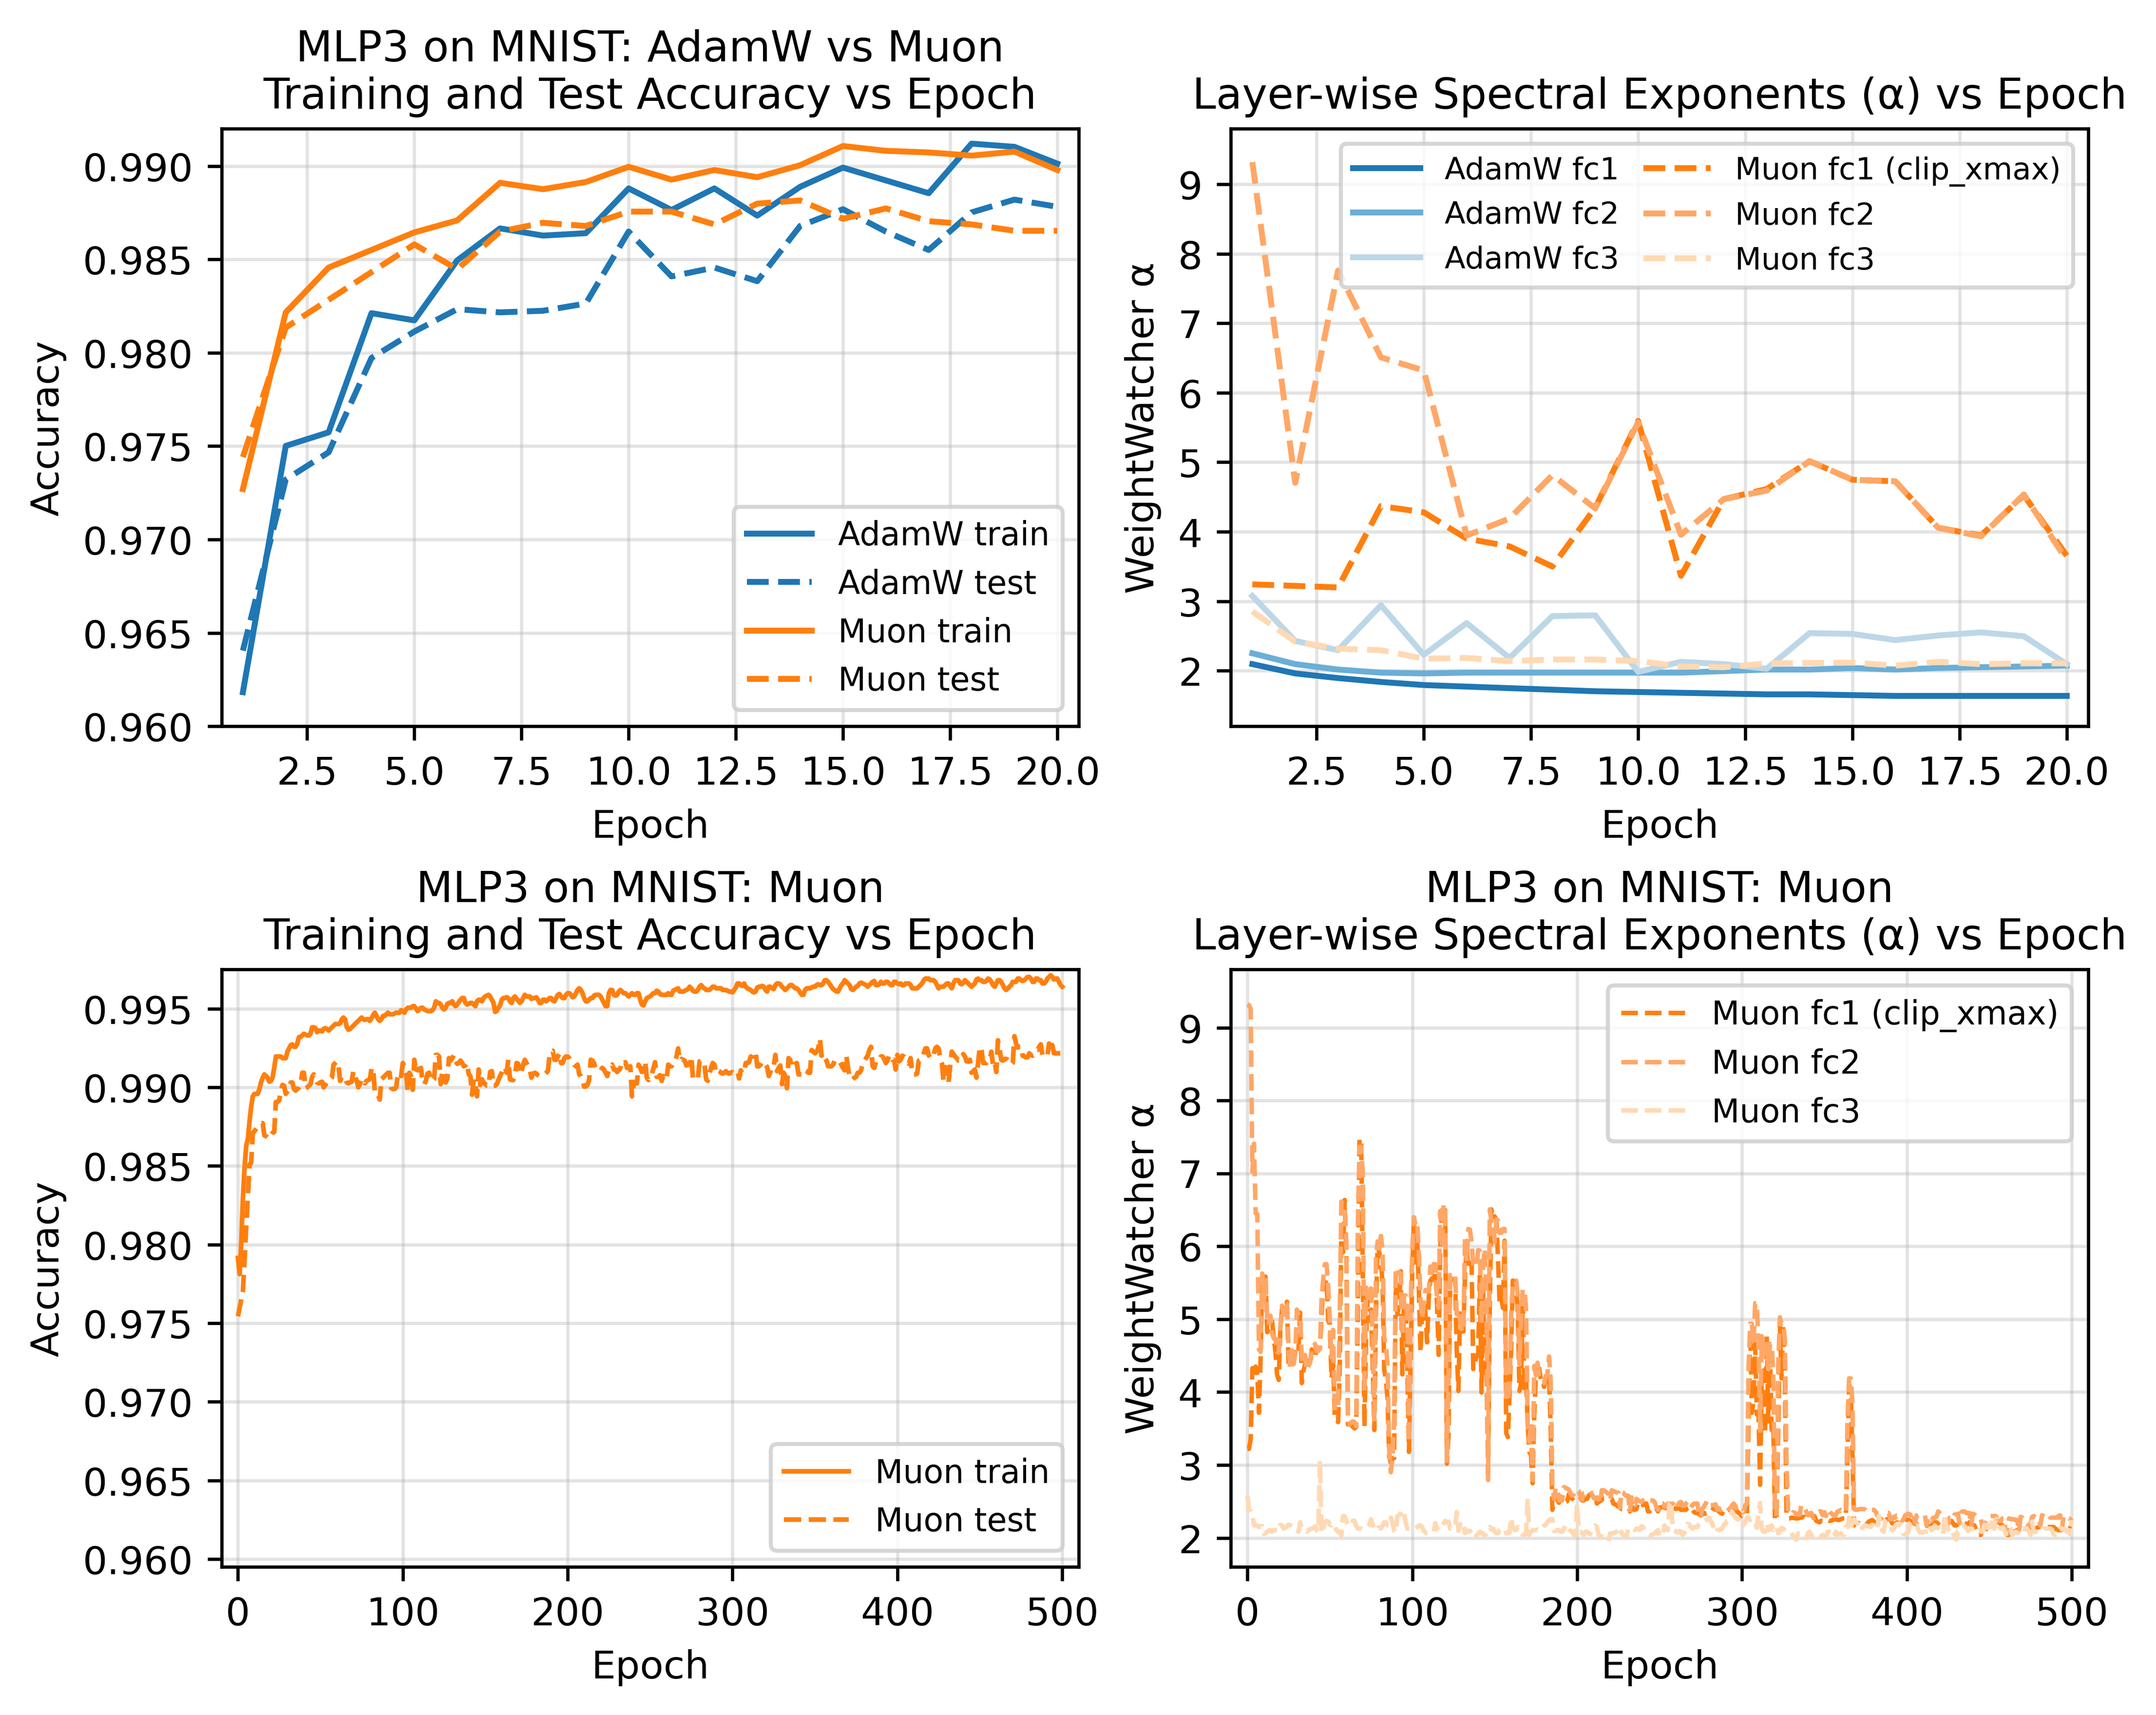
\includegraphics[width=0.8\textwidth]{figures/figure9_mnist_optimizer_comparison_panelgrid.png}
\caption{\textbf{MNIST optimizer comparison: AdamW versus Muon.}
Same three-layer MNIST MLP trained with AdamW and Muon.
Short-horizon panel compares early epochs; long-horizon panel tracks the Muon $\alpha_{\ell}(t)\rightarrow 2$.}
\label{fig:mnist_optimizer_comparison}
\end{figure*}

\begin{tcolorbox}[marginalbox,title=\textbf{14. Muon test}]
\begin{itemize}
\item \textbf{Compare:} AdamW and Muon.
\item \textbf{Model:} three-layer MNIST MLP.
\item \textbf{Measure:} layerwise \(\alpha(t)\).
\end{itemize}
\takeaway{Muon changes the spectral route.}
\end{tcolorbox}

The Muon test asks whether update geometry changes the spectral route.  The controlled model is a three-layer MNIST MLP, described
in the Appendix~\ref{app:optimizer_experiments}.  The comparison holds the data, model, and diagnostics fixed.  Only the matrix-valued update rule changes: AdamW~\cite{LoshchilovHutter2019} is compared to Muon.  At checkpoints, \WW~fits the HTSR exponent of each fully connected layer
\begin{equation}
        \alpha_\ell(t),
        \qquad
        \ell\in\{\mathrm{FC1},\mathrm{FC2},\mathrm{FC3}\}.
\end{equation}


Figure~\ref{fig:mnist_optimizer_comparison} compares results for Muon agains AdamW~\cite{LoshchilovHutter2019}.;
it depicts the test and training accuracies and the layerwise $\alpha_{\ell}(t)$ per epoch.
The top panels compare AdamW and Muon over the first twenty $(20)$ epochs, while the bottom panels
track Muon for five-hundred $(500)$ epochs.

Consider the top panels first.
AdamW reaches high train and test accuracy more slowly than Muon, but reaches a comparable range after twenty $(20)$ epochs.
The AdamW and Muon layerwise $\alpha_\ell(t)$ curves behave very differently over these early epochs.
For AdamW, all layer $\alpha_\ell(t)$ values drop quickly. FC2 and FC3 approach the optimal value $\alpha=2$,
but FC1 immediately collapses below $2.0$ and remains trapped in the proposed overfitting regime, even as accuracy increases.
In contrast, only Muon's FC3 layer approaches $\alpha=2$ quickly,
while FC1 and FC2 fluctuate at first, and then remain near $\alpha=4$.

The bottom panels show Muon over very long-horizon runs.
Neither Muon training accuracy nor test accuracy drops; both increase slowly and asymptotically.
Muon FC1 and FC2 track each other, first fluctuating strongly with $\alpha_\ell(t)\in[3,6]$.
Eventually, however, all layer values satisfy $\alpha_\ell(t)\rightarrow 2$, again very slowly.

This comparison is intentionally untuned. We made no attempt to optimize learning rates or make Muon win the MNIST benchmark.

In summary, AdamW overfits immediately, while Muon approaches the proposed RG fixed point
asymptotically slowly.  This is consistent with Muon removing the
proposed RG redundant scale directions, and could be associated with RG \emph{critical slowing down}.
\clearpage
\newpage
\subsection{WW-PGD test}
\label{sxn:wwpgd_empirical_test}

\begin{tcolorbox}[marginalbox,title=\textbf{15. WW-PGD test}]
\begin{itemize}
\item \textbf{Compare:} AdamW and AdamW+WW-PGD.
\item \textbf{Run:} 35 epochs, five seeds.
\item \textbf{Measure:} FC1--FC3 exponents.
\end{itemize}
\takeaway{WW-PGD stabilizes \(\alpha\) near two.}
\end{tcolorbox}

The WW-PGD test asks whether the proposed optimizer can reduce AdamW overfitting by preventing the layer exponents
$\alpha_\ell(t)$ from dropping below $2$, while simultaneously helping all layers approach the proposed RG fixed point
$\alpha\simeq 2$. The experiment is similar to the Muon test (Section~\ref{sxn:muon_empirical_test}), and is described in
Appendix~\ref{app:optimizer_experiments}.

The WW-PGD condition uses the same AdamW minibatch optimizer,
but applies the epoch-boundary retraction in Eq.~\eqref{eq:wwpgd_outer_map}.
The experiment runs for 35 epochs and five independent runs. The WW-PGD hyperparameters are
\begin{equation}
        q=1,
        \qquad
        \eta_B=0.5,
        \qquad
        \eta_C=0.25,
\end{equation}
with zero warmup and a five-epoch homotopy ramp.

The experimental results are visually clear.
At each epoch, \WW~logs the HTSR exponent $\alpha_\ell(t)$.
The plotted curves report the mean and standard deviation of
\begin{equation}
        \alpha_\ell(t),
        \qquad
        \ell\in\{\mathrm{FC1},\mathrm{FC2},\mathrm{FC3}\}.
\end{equation}

Figure~\ref{fig:wwpgd_alpha_per_layer} shows the layerwise results.
AdamW alone lets the $\alpha_\ell(t)$ exponents separate by layer.
As in the Muon comparison, the FC1 exponent satisfies $\alpha_\ell(t)<2$ throughout most of training, while the FC2 exponent satisfies $\alpha_\ell(t)\geq2$.
The FC3 exponent satisfies $\alpha_\ell(t)\gg2$; however, this does not materially change the overall conclusions.

WW-PGD improves the layer $\alpha_\ell(t)$ for all layers, while keeping the training and test accuracies close to, or only slightly below, the baseline AdamW results.

\begin{figure}[t]
  \centering
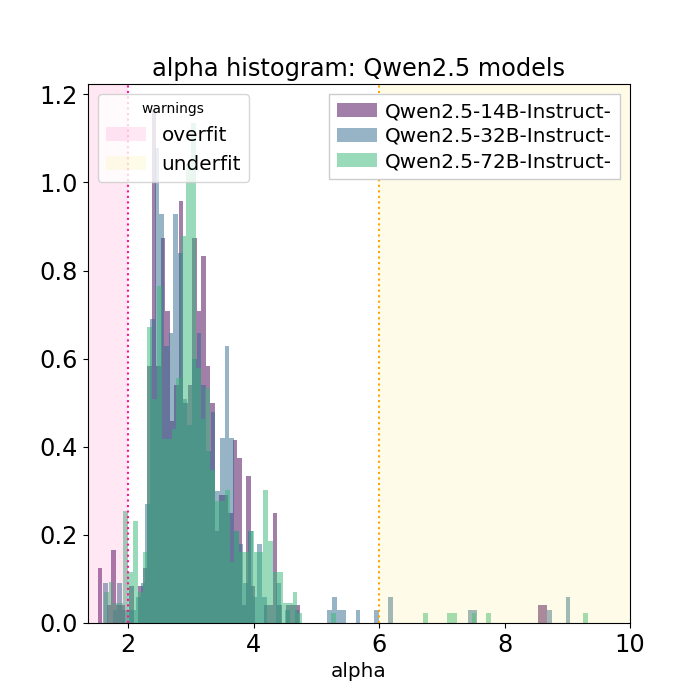
\includegraphics[width=\linewidth]{figures/wwpgd_alpha_readable.png}\\[-0.35em]
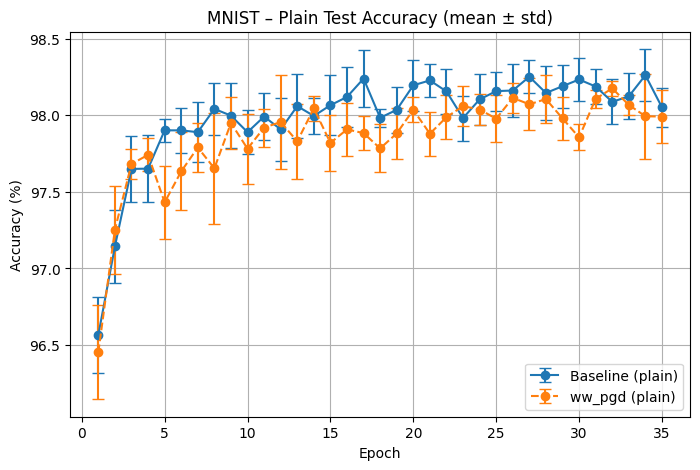
\includegraphics[width=\linewidth]{figures/wwpgd_accuracy_readable.png}
\caption{\textbf{WW-PGD stabilizes layerwise HTSR exponents while preserving test accuracy.}
A three-layer MNIST MLP is trained with AdamW alone or AdamW plus WW-PGD. Top: layerwise fitted HTSR exponents for FC1--FC3. Bottom: ordinary MNIST test accuracy. Curves show mean \(\pm\) standard deviation across five runs.}
\label{fig:wwpgd_alpha_per_layer}
\end{figure}

WW-PGD does not win by changing the task optimizer or accelerating convergence; in fact, it is slightly slower.
The minibatch AdamW step is unchanged, and WW-PGD acts only at the epoch boundary.
Still, the ordinary MNIST test accuracy remains within the visible run-to-run variation in the WW-PGD results.

The convergence to the proposed RG optimal boundary is much faster than with Muon. This is the key takeaway.
Muon normalizes the update, but it does not inspect the layer spectrum. WW-PGD does inspect the spectrum.
It selects the retained tail and retracts that tail toward the RG boundary.
This makes WW-PGD a direct finite-step test of the spectral-RG optimizer hypothesis.
Appendix~\ref{app:optimizer_experiments} lists the default settings and links to the reproduction notebooks.

Together, the two empirical tests separate the roles of the optimizers.
Muon shows that removing product scale from updates changes spectral dynamics.
WW-PGD then adds the missing state-space operation: measure the layer spectrum, select the retained tail, and retract that tail toward the RG boundary
$\alpha\simeq 2$ for each layer.

\paragraph{Repairing an anti-grokking checkpoint.}
A more constructive question is whether a model that has already entered an overfitted or anti-grokking state can be fixed.
In ongoing work with H.~K. Prakash, we take an anti-grokking checkpoint from the long-horizon grokking experiments of Prakash and Martin~\cite{PrakashMartinTraps2026} and continue training from that exact state using AdamW, Muon, and WW-PGD.
AdamW and Muon are optimizer controls: they resume learning from the same checkpoint, but they do not directly inspect the fitted spectral tail.
WW-PGD uses \WW{} diagnostics as state variables, selects the retained tail, and retracts that tail toward the RG boundary $\alpha\simeq2$.
Preliminary results, shown in Figure~\ref{fig:wwpgd_antigrokking_repair}, suggest that WW-PGD may function as a repair map, not only as a preventative spectral regularizer.
This experiment is ongoing and will be reported separately; it is included here as future work rather than as evidence for the main empirical claims of this paper.

\begin{figure}[t]
  \centering
  \includegraphics[width=\linewidth]{figures/fixed_grok.png}
  \caption{\textbf{Future work: WW-PGD repair from an anti-grokking checkpoint.}
  Preliminary continual-learning runs start from the same anti-grokking checkpoint from the long-horizon grokking study of Prakash and Martin~\cite{PrakashMartinTraps2026}.
  AdamW, Muon, and WW-PGD are then continued from that checkpoint.
  WW-PGD is designed to inspect the retained spectral tail and retract it toward the RG boundary $\alpha\simeq2$.
  This panel is included as an ongoing-work diagnostic, not as a main empirical result.}
  \label{fig:wwpgd_antigrokking_repair}
\end{figure}
\clearpage
\section{Implications of Universality}
\label{sec:implications}

Universality is a statement about the coarse-grained endpoint of learning, not about the microscopic form of the algorithm. Neural networks, boosted trees, kernel methods, and matrix factorization procedures use different update rules, but each can induce an effective correlation structure on the data~\cite{GalluccioBouchaudPotters1998}. Figure~\ref{fig:rg-universality-flow} represents that structure by effective couplings $\widetilde g_i(\mu)$ that flow with RG scale $\mu$. The RG question is whether these spectra approach a common critical surface and candidate fixed point $g^\star$.

\begin{figure}[!t]
\centering
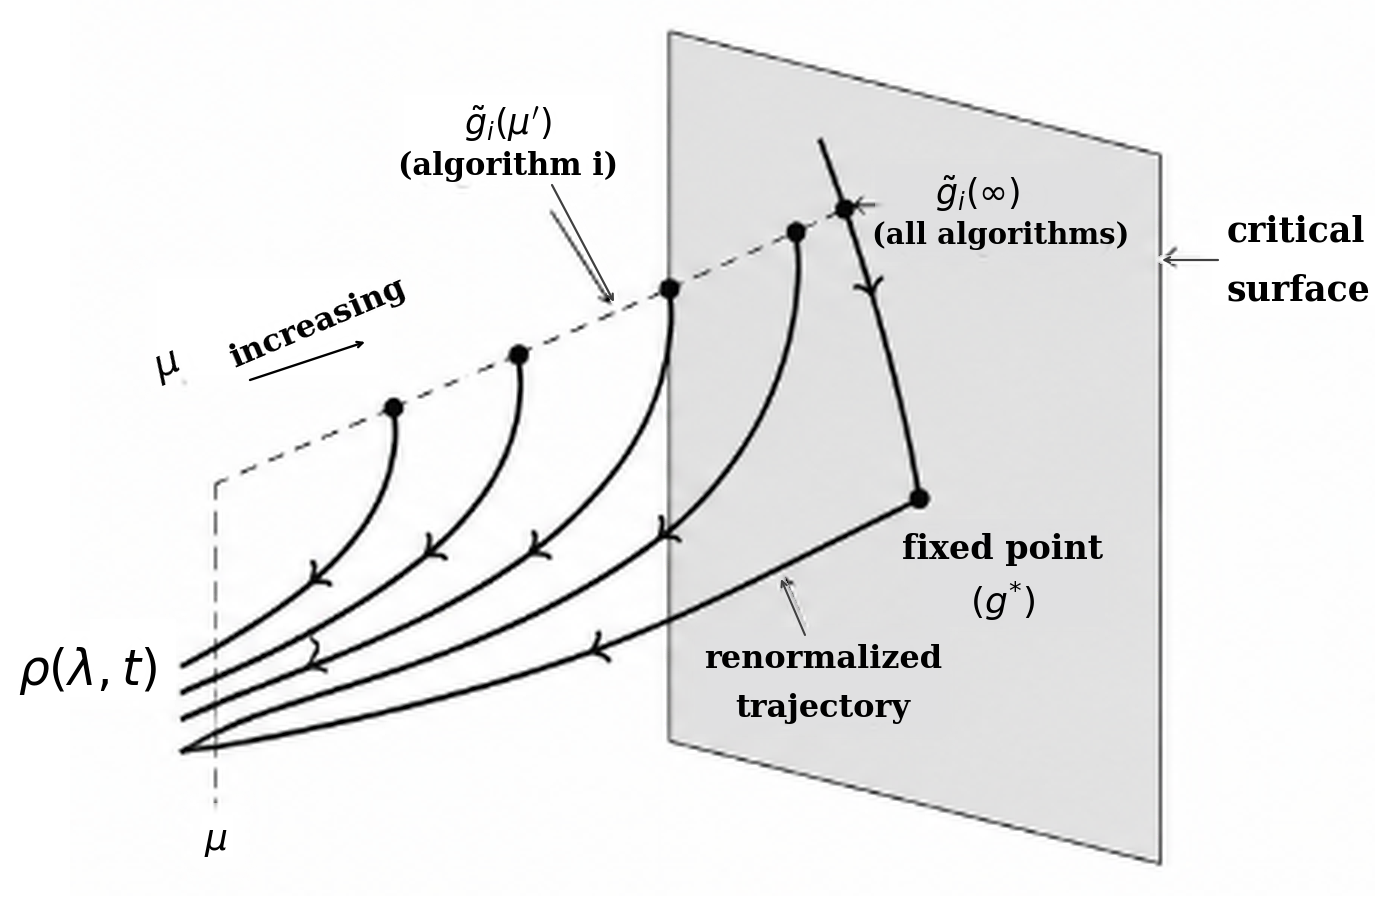
\includegraphics[width=\columnwidth]{figures/rg_universality_flow.png}
\caption{RG flow in the space of effective correlations. Different nonlinear learning algorithms follow different microscopic trajectories, but coarse-graining can suppress irrelevant directions and carry retained spectral structure toward a candidate fixed point. Candidate universal quantities are read off near the fixed point, not from the microscopic update rule.}
\label{fig:rg-universality-flow}
\end{figure}



\begin{tcolorbox}[marginalbox,title=\textbf{16. Universality of learning algorithms}]
Universality asks whether different nonlinear learners can flow to the same coarse-grained candidate spectral fixed point.

\begin{itemize}
\item Nonlinear learning algorithms can be linearized near their fixed points.
\item Spectra, not parameters, may characterize the optimal conditions.
\item Self-averaging bulk modes support transfer.
\item Non-self-averaging modes reveal dominant atypical structure that causes overfitting.
\item XGBoost is a conjectural test case.
\end{itemize}

\takeaway{RG universality means different algorithms may share a candidate fixed-point spectrum.}

\end{tcolorbox}

The RG claim is local. A learner can be nonlinear away from convergence. Near a stable endpoint, its coarse-grained flow can be linearized in a few spectral coordinates $\widetilde g_i$. In Figure~\ref{fig:rg-universality-flow}, the renormalized trajectories bend toward the same critical surface. The stable directions define the universality class, and the fixed point $g^\star$ defines the universal spectral observables.

Near the proposed RG fixed point, the eigenspectrum of the linearized learner carries the invariant information in the retained correlation operator. Parameters change with architecture, but the proposed ERG point may be universal. A non-neural learner needs its own effective correlation operator. Universality becomes testable only after that operator and its $\widetilde g_i$ coordinates are defined.

Self-averaging is another universal property. The bulk spectral averages should stabilize across samples, initializations, and checkpoints.  Non-self-averaging modes should concentrate into a few dominant elements in the spectral tail.
Tail modes are not automatically bad. They become risky when a few directions carry too much trace-law gain,
causing correlation traps to form and/or $\alpha < 2$.

Neural networks give the direct case. Different depths, widths, initializations, and optimizers can produce similar endpoint spectra. The shared object is the normalized effective correlation spectrum. This view also reframes optimizer design. A good optimizer should reduce loss while steering the spectrum toward a self-averaging marginal boundary between
optimality and overfitting, with $\alpha\simeq 2$ as a candidate universal spectral exponent.

XGBoost gives a plausible extension~\cite{ChenGuestrin2016}. Boosting has no dense layer weight matrix, so the current layer-specific theory does not apply directly. Still, each tree changes the residuals and the prediction function. Those updates induce a data-data correlation structure in prediction space. A practical test would form a centered Gram operator from tree contributions or prediction increments, normalize its scale, and track its spectrum across boosting rounds.
Early work (not shown) suggests this is possible and future work will explore applying the RG theory and the \WW~tool to XGBoost models.

Universality does not say that all algorithms compute the same function. It says that successful learners may share the same coarse-grained spectral organization. Generalization would then depend less on update details and more on self-averaging, marginality, and controlled dominant modes.


More broadly, universality suggests transferability. In semi-empirical electronic-structure theory, transferable parameters work because different molecules can share the same effective valence-space structure. Martin and Freed tested this idea by deriving semiempirical $\pi$-electron parameters from ab initio effective valence-shell Hamiltonians and studying when those parameters transfer across related molecules \cite{MartinFreed1994I,Martin1996SchiffBases,Martin1996LargeSchiffBases}.
The analogy here is direct. If learned correlation spectra have candidate universal fixed-point structure, then useful spectral parameters may transfer across related models, tasks, optimizers, and even algorithm families. Transferability would then come from the effective correlation space, not from the microscopic implementation.


\clearpage
\section{Conclusions}
\label{sxn:conclusions}

This paper gives an RG theory of NN layer convergence, integrating the older phenomenological HTSR approach and the more recently developed
SETOL theory. HTSR supplies the empirical fact: strong layers often develop heavy-tailed spectra near $\alpha\simeq2$. SETOL supplies the trace-log condition: remove arbitrary layer scale and study the retained effective correlation space. The main claim is that these two pictures meet at the same spectral endpoint.

The value $\alpha=2$ has two meanings. Statistically, it marks the boundary between stable bulk-supported learning and domination by a few extreme eigencomponents. RG scale counting gives the same boundary. At $\alpha=2$, each logarithmic spectral shell contributes comparable trace-law gain. This agreement makes $\alpha\simeq2$ a critical boundary, not just a fitted number.

The fixed point is layerwise. Each dense layer has its own retained spectrum, trace-log scale, and dominant-tail burden. A trained network is therefore not one monolithic fixed point. It is a coordinated state in which many layers approach compatible spectral endpoints.

The practical diagnostic is spectral. A good layer should keep useful correlation gain spread across many retained eigencomponents. A bad layer can concentrate too much gain in a few dominant tail modes. The trace-log condition removes scale. The fitted tail measures shape. The dominant-tail fraction tests whether the layer remains self-averaging.

The optimizer message is also spectral. Raw optimizers can spend update norm on scale-only motion. A better optimizer should reduce loss while steering the retained spectrum toward the correlated, self-averaging branch. This view suggests why matrix-aware optimizers such as Muon are relevant. It also suggests new optimizer designs based on trace-log geometry.

The WeightWatcher message becomes sharper. The fitted exponent $\alpha$, the trace-log coordinate, ECS--tail alignment, trap counts, participation counts, and dominant-tail burden are not isolated heuristics. They are RG observables of the same layerwise spectral flow. They can be measured from weights alone, without labels, gradients, or test data.

The empirical program is direct. Track these observables across checkpoints. Compare them across optimizers. Ask whether held-out performance improves when the spectrum approaches the marginal boundary and degrades when dominant modes take over. This turns the RG picture into a falsifiable diagnostic program.

The limitations are direct. This paper does not prove convergence of SGD, AdamW, or Muon to the proposed spectral fixed point. It proposes an operational RG interpretation of retained layer spectra and connects that interpretation to HTSR and SETOL diagnostics. The evidence supports this picture on the models studied here, but it does not establish universality across all architectures, datasets, optimizers, or nonlinear learners.

The broader implication is transferability. Semi-empirical electronic-structure theory uses transferable parameters because related molecules share effective valence-space structure. The analogy here is direct. If learned correlation spectra have candidate universal fixed-point structure, then useful spectral parameters may transfer across related models, tasks, optimizers, and algorithm families.

The final message is simple. Learning is not only loss minimization. Learning is spectral organization. Good layers move toward a candidate correlated fixed point where scale is removed, the tail is balanced, and trace-law gain remains self-averaging.


\begin{tcolorbox}[marginalbox,title=\textbf{17. The theory in one pass}]
Dense layers learn by moving their spectra.
\begin{itemize}
\item HTSR observes heavy-tailed spectra near $\alpha\simeq2$.
\item SETOL connects heavy-tailed layer spectra to model accuracy (called layer quality), and derives the ERG trace-log laws.
\item Self-averaging explains why $\alpha=2$ is optimal and $\alpha<2$ is risky.
\item RG scale counting explains why $\alpha=2$ is marginal, suggesting a candidate universal spectral exponent.
\item Optimizers should reduce scale-only motion and move toward the proposed ERG fixed point.
\item The theory may be extensible to XGBoost and related algorithms:
  $\alpha=2$  and $\Tr{\log\tilde{\mathbf{X}}}=0$.
\end{itemize}
\takeaway{Keep the learned tail, remove its scale, and test whether the retained layer stays balanced.}
\end{tcolorbox}

\section*{Acknowledgments}
The author thanks H.~K. Prakash for ongoing collaboration on long-horizon grokking, anti-grokking diagnostics, and the preliminary WW-PGD repair experiments discussed here as future work.

\clearpage
\onecolumn
\thispagestyle{plain}
\begin{center}
\vspace*{-1.0em}
\setlength{\tabcolsep}{3pt}
\renewcommand{\arraystretch}{1.04}
\captionof{table}{Notation and conventions used in this report.}
\label{tab:notation-conventions}
\resizebox{\textwidth}{!}{%
\begin{tabular}{@{}lll@{}}
\toprule
Group & Symbol & Meaning \\
\midrule
Layer & $\W\in\mathbb R^{N\times M}$, $N\ge M$ & Dense-layer weights. \\
Layer & $\X=N^{-1}\W^T\W$ & Layer correlation operator. \\
Layer & $\lambda_i>0$, $\Splus=\{i:\lambda_i>0\}$ & Positive spectral support. \\
PL tail & $\rho_{\rm tail}(\lambda)\sim\lambda^{-\alpha}$ & HTSR tail; fitted exponent $\alpha$. \\
PL tail & $\TPL$, $\TPL^\star$ & CSN-selected PL window. \\
ECS & $\Rell\subseteq\Splus$, $\Mred=|\Rell|$ & Retained ECS and size. \\
ECS & $\RECS^\star$ & Stabilized SETOL ECS. \\
Alignment & $\RECS^\star\simeq\TPL^\star$ & SETOL--HTSR window match. \\
Trace-log & $\XR=\U_{\Rell}^T\X\U_{\Rell}$ & ECS-restricted operator. \\
Trace-log & $\lambda_g^{(\Rell)}=\exp(\Mred^{-1}\sum_{i\in\Rell}\log\lambda_i)$ & Raw retained geometric mean. \\
Trace-log & $\Xtilde_{\Rell}=\XR/\lambda_g^{(\Rell)}$, $\widetilde\lambda_i=\lambda_i/\lambda_g^{(\Rell)}$ & Unit-geometric-mean ECS. \\
Trace-log & $\Tr\log\Xtilde_{\Rell}=\sum_{i\in\Rell}\log\widetilde\lambda_i=0$ & Product-scale fixing. \\
SETOL & $\X_{\Rell}^{\rm SETOL}=\XR/M$, $\widetilde\lambda_i^{\rm SETOL}=\lambda_i/M$ & Width-$M$ normalization. \\
Energy & $E_+=M^{-1}\Tr\X$ & Full trace-law gain. \\
Energy & $\Ered=\Mred^{-1}\sum_{i\in\Rell}\lambda_i=\int\lambda\rhohat_{\Rell}(\lambda)d\lambda$ & Retained first moment. \\
Tail & $\phi_k^R=\sum_{j=1}^k\lambda_{R(j)}/\sum_{i\in\Rell}\lambda_i$ & Top-$k$ gain fraction. \\
Tail & $M_{\rm tr}^R=(\sum_{i\in\Rell}\lambda_i)^2/\sum_{i\in\Rell}\lambda_i^2$ & Effective contributor count. \\
Scale & $x=\log\lambda$, $[\Lambda,b\Lambda]$ & Log coordinate and shell. \\
Scale & $G_E(\Lambda,b)=\int_{\Lambda}^{b\Lambda}\lambda\rhohat_{\Rell}(\lambda)d\lambda$ & Band trace-law gain. \\
Scale & $g_E(z)=d\overline E/d\log z$, $z=\lambda/\lambda_g^{(\Rell)}$ & Scale-removed shell gain. \\
Beta & $\beta_E(g_E)=d g_E/d\log\lambda=(2-\alpha)g_E$ & Leading PL scale derivative. \\
Marginal & $y_E=2-\alpha=0$ & Log-band balance. \\
Fixed point & $\mathcal R_{\rm RG}[\rho^\star]=\rho^\star$ & Normalized spectral fixed point. \\
Branch & $\Fzero$, $\Fhtsr$ & RG spectral branches. \\
Branch & $\Fzero:g_E^\star=0$ & Trivial/random-like branch. \\
Branch & $\Fhtsr:0<g_E^\star<\infty,\ \alpha\simeq2,\ \RECS^\star\simeq\TPL^\star$ & Empirical HTSR/SETOL branch. \\
Quality & $\overline Q_{\rm NN}$, $\overline Q_\ell$ & Model and layer quality. \\
Optimizer & $A_{\Rell}=\U_{\Rell}\XR^{-1}\U_{\Rell}^T$, $G_T=\nabla_W T_{\Rell}$ & Trace-log gradient objects. \\
Optimizer & $\Delta\W_\perp$ & Trace-log projected update. \\
WW-PGD & $\Tell$, $m=|\Tell|$ & Selected tail and size. \\
WW-PGD & $\lambda_k^\star=A k^{-q}$, $q=1$ & Rank-order tail target. \\
WW-PGD & $\eta_B,\eta_C,h_e$ & Blend, Cayley, homotopy factors. \\
\bottomrule
\end{tabular}}
\end{center}
\clearpage

\appendix
\section{Optimizer experiment details}
\label{app:optimizer_experiments}
\small

This appendix records the optimizer protocols. Both tests use MNIST and the same three-layer MLP, $784\rightarrow512\rightarrow512\rightarrow10$, with ReLU nonlinearities. The linear layers are logged as FC1--FC3. MNIST inputs use mean $0.1307$ and standard deviation $0.3081$. At checkpoints, \WW{} records the fitted HTSR exponent $\alpha$ and the tail diagnostics for each fully connected layer.

\paragraph{Reproduction notebooks.}
The Muon panel uses the public notebooks \href{https://github.com/CalculatedContent/WeightWatcher-Examples/blob/main/AdamWvsMuon.ipynb}{AdamWvsMuon.ipynb}, \href{https://github.com/CalculatedContent/WeightWatcher-Examples/blob/main/MLP3-MNIST-AdamW.ipynb}{MLP3-MNIST-AdamW.ipynb}, and \href{https://github.com/CalculatedContent/WeightWatcher-Examples/blob/main/MLP3-MNIST-Muon.ipynb}{MLP3-MNIST-Muon.ipynb}. The WW-PGD wrapper is reproduced from \href{https://github.com/CalculatedContent/WW_PGD/blob/main/WW_PGD_QuickStart.ipynb}{WW\_PGD\_QuickStart.ipynb}. The plotted curves use the settings below.

\paragraph{Muon test.}
The Muon test compares AdamW and Muon on the same model and data. AdamW gives the baseline trajectory. Muon is applied to matrix-valued hidden-layer updates. Scalar, bias, and other non-matrix parameters are handled by the associated base optimizer. The short-horizon panel tracks the early optimizer separation. The long-horizon panel tracks the slower Muon approach over hundreds of epochs. Training and test accuracy are logged with the layerwise curves $\alpha(t)$, $\ell\in\{\mathrm{FC1},\mathrm{FC2},\mathrm{FC3}\}$.

\paragraph{WW-PGD test.}
The WW-PGD test compares AdamW with AdamW+WW-PGD. The minibatch optimizer is fixed. The batch size is $128$. AdamW uses learning rate $10^{-3}$. Gradients are clipped to norm $1.0$. The main run uses $35$ epochs and five independent runs. At every epoch, \WW{} analyzes the model with \texttt{detX=True}, \texttt{randomize=False}, and \texttt{plot=False}. WW-PGD applies one epoch-boundary spectral retraction with \texttt{min\_tail}=5, $q=1$, $\eta_B=0.5$, $\eta_C=0.25$, \texttt{use\_detx=True}, \texttt{warmup\_epochs}=0, \texttt{ramp\_epochs}=5, and \texttt{enable\_trap\_pgd=False}.

\paragraph{WW-PGD correction.}
For each eligible layer, WW-PGD forms $\lambda_i=s_i^2$ and selects the retained tail from \WW{} diagnostics such as $\lambda_{\min}$ and \texttt{detX\_num}. It sorts the tail eigenvalues in decreasing order and uses the target $\lambda_k^\star=A k^{-1}$. The amplitude $A$ preserves the retained tail trace-log. The moved tail is recentered, reconstructed with the original singular vectors, and blended back into the post-AdamW layer. The standard test loader uses ordinary MNIST. The perturbed loader uses random rotation by $7^\circ$, random translation by $3\%$, small Gaussian blur, and no horizontal flip.

\clearpage
\twocolumn
%\enlargethispage{3\baselineskip}
\begin{thebibliography}{99}
\footnotesize\setlength{\itemsep}{0pt}\setlength{\parskip}{0pt}

\bibitem{MartinMahoneyICML2019}
M.~W. Mahoney and C.~H. Martin, ``Traditional and heavy-tailed self-regularization in neural network models,'' \emph{Proceedings of the 36th International Conference on Machine Learning}, PMLR 97:4284--4293, 2019; arXiv:1901.08276.

\bibitem{MartinMahoneyJMLR2021}
C.~H. Martin and M.~W. Mahoney, ``Implicit self-regularization in deep neural networks: Evidence from random matrix theory and implications for learning,'' \emph{Journal of Machine Learning Research} 22(165):1--73, 2021. \url{https://jmlr.org/papers/v22/20-410.html}.

\bibitem{MartinPengMahoney2021}
  C.~H. Martin, T.~S. Peng, and M.~W. Mahoney, ``Predicting trends in the quality of state-of-the-art neural networks without access to training or testing data,'' \emph{Nature Communications} 12, 4122, 2021. DOI: 10.1038/s41467-021-24025-8.

\bibitem{MartinMahoney2020SDM}
C.~H. Martin and M.~W. Mahoney,
``Heavy-Tailed Universality Predicts Trends in Test Accuracies for Very Large Pre-Trained Deep Neural Networks,''
in \emph{Proceedings of the 2020 SIAM International Conference on Data Mining},
SIAM, 2020, pp.~505--513.
doi: \texttt{10.1137/1.9781611976236.57}.

\bibitem{MartinHinrichsSETOL2025}
C.~H. Martin and C.~Hinrichs, ``SETOL: A semi-empirical theory of (deep) learning,'' arXiv:2507.17912, 2025.

\bibitem{PrakashMartinTraps2026}
H.~K. Prakash and C.~H. Martin, ``Detecting overfitting in neural networks during long-horizon grokking using random matrix theory,'' arXiv:2605.12394, 2026.


\bibitem{PrakashMartinLateCollapse2026}
H.~K. Prakash and C.~H. Martin, ``Late-stage generalization collapse in grokking: Detecting anti-grokking with WeightWatcher,'' arXiv:2602.02859, 2026.

\bibitem{WeightWatcherTool}
  C.~H. Martin, ``WeightWatcher: An open-source diagnostic tool for deep neural networks,'' GitHub repository, \url{https://github.com/CalculatedContent/WeightWatcher}.

\bibitem{MarchenkoPastur1967}
V. A. Marchenko and L. A. Pastur,
``Distribution of eigenvalues for some sets of random matrices,''
\emph{Mathematics of the USSR-Sbornik} 1, 457--483, 1967. DOI: 10.1070/SM1967v001n04ABEH001994.

\bibitem{TracyWidom1996}
C. A. Tracy and H. Widom,
``On orthogonal and symplectic matrix ensembles,''
\emph{Communications in Mathematical Physics} 177, 727--754, 1996. DOI: 10.1007/BF02099545; arXiv:solv-int/9509007.

\bibitem{SeungSompolinskyTishby1992}
H. S. Seung, H. Sompolinsky, and N. Tishby,
``Statistical mechanics of learning from examples,''
\emph{Physical Review A} 45, 6056--6091, 1992.
DOI: 10.1103/PhysRevA.45.6056.

\bibitem{CizeauBouchaud1994}
P.~Cizeau and J.-P. Bouchaud, ``Theory of L\'evy matrices,'' \emph{Physical Review E} 50, 1810--1822, 1994. DOI: 10.1103/PhysRevE.50.1810.

\bibitem{PottersBouchaud2020}
M.~Potters and J.-P.~Bouchaud, \emph{A First Course in Random Matrix Theory: For Physicists, Engineers and Data Scientists}, Cambridge University Press, 2020.

\bibitem{GalluccioBouchaudPotters1998}
S.~Galluccio, J.-P.~Bouchaud, and M.~Potters, ``Rational decisions, random matrices and spin glasses,'' \emph{Physica A} 259, 449--456, 1998. DOI: 10.1016/S0378-4371(98)00332-X; arXiv:cond-mat/9801209.

\bibitem{Zee1996}
A.~Zee, ``Law of addition in random matrix theory,'' \emph{Nuclear Physics B} 474, 726--744, 1996. DOI: 10.1016/0550-3213(96)00276-3; arXiv:cond-mat/9602146.

\bibitem{WilsonKogut1974}
K. G. Wilson and J. B. Kogut, ``The renormalization group and the epsilon expansion,'' \emph{Physics Reports} 12, 75--199, 1974. DOI: 10.1016/0370-1573(74)90023-4.

\bibitem{Polchinski1984}
J.~Polchinski, ``Renormalization and effective Lagrangians,'' \emph{Nuclear Physics B} 231, 269--295, 1984. DOI: 10.1016/0550-3213(84)90287-6.

\bibitem{Clauset2009}
A.~Clauset, C.~R. Shalizi, and M.~E.~J. Newman, ``Power-law distributions in empirical data,'' \emph{SIAM Review} 51, 661--703, 2009. DOI: 10.1137/070710111.

\bibitem{LoshchilovHutter2019}
I.~Loshchilov and F.~Hutter, ``Decoupled weight decay regularization,'' \emph{International Conference on Learning Representations}, 2019; arXiv:1711.05101.

\bibitem{JordanMuon2024}
K.~Jordan, Y.~Jin, V.~Boza, J.~You, F.~Cesista, L.~Newhouse, and J.~Bernstein, ``Muon: An optimizer for hidden layers in neural networks,'' online technical note, 2024, URL: \url{https://kellerjordan.github.io/posts/muon/}.

\bibitem{LiuMuonScalable2025}
J.~Liu et al., ``Muon is scalable for LLM training,'' arXiv:2502.16982, 2025.

\bibitem{BernsteinNewhouse2025}
J.~Bernstein and L.~Newhouse, ``Modular Duality in Deep Learning,'' in \emph{Proceedings of the 42nd International Conference on Machine Learning}, PMLR 267:3920--3930, 2025; arXiv:2410.21265.

\bibitem{MartinFreed1994I}
C.~H. Martin and K.~F. Freed,
``Ab initio computation of semiempirical $\pi$-electron methods. I.
Constrained, transferable valence spaces in $\mathcal H^\nu$ calculations,''
\emph{Journal of Chemical Physics} \textbf{100}, 7454--7470, 1994.
DOI: 10.1063/1.466889.

\bibitem{Martin1996SchiffBases}
C.~H. Martin,
``Highly accurate ab initio $\pi$-electron Hamiltonians for small protonated Schiff bases,''
\emph{Journal of Physical Chemistry} \textbf{100}, 14310--14315, 1996.
DOI: 10.1021/jp960617w.

\bibitem{Martin1996LargeSchiffBases}
C.~H. Martin,
``Redesigning semiempirical-like $\pi$-electron theory with second order effective valence shell Hamiltonian ($H^\nu$) theory: Application to large protonated Schiff bases,''
\emph{Chemical Physics Letters} \textbf{257}, 229--237, 1996.
DOI: 10.1016/0009-2614(96)00548-9.

\bibitem{ChenGuestrin2016}
T. Chen and C. Guestrin,
``XGBoost: A scalable tree boosting system,''
in \emph{Proceedings of the 22nd ACM SIGKDD International Conference on Knowledge Discovery and Data Mining},
785--794, 2016. DOI: 10.1145/2939672.2939785; arXiv:1603.02754.
\end{thebibliography}

\end{document}
